\documentclass[10pt]{article}
\usepackage{helvet}

\long\def\comment#1{}

\long\def\commenta#1{{\bf **Amy: #1**}}
\long\def\commentj#1{{\bf **Joe: #1**}}
\long\def\commentm#1{{\bf **Michael: #1**}} 

%\long\def\commenta#1{}
%\long\def\commentm#1{}

\usepackage{bm}
\usepackage{url}
\usepackage{hyperref}
\usepackage{epsfig}
\usepackage{wrapfig}
\usepackage{fullpage}
\usepackage{amsmath}
\usepackage{mathsymb}
\usepackage{caption}
\usepackage{subcaption}

\usepackage{graphicx}

\usepackage{algorithm}
\usepackage{algpseudocode}

\usepackage{tikz}
\usetikzlibrary{bayesnet}

\usepackage{defs}
\usepackage{macros}

\newcommand*{\Scale}[2][4]{\scalebox{#1}{$#2$}}%
\newcommand*{\Resize}[2]{\resizebox{#1}{!}{$#2$}}%

\newcommand{\jmnote}[1]{\textcolor{Green}{\textbf{[JM: #1]}}}

\newcommand{\mydef}[1]{\textbf{\boldmath{#1}}}

\newcommand{\up}{-2.5mm}
\newcommand{\down}{1mm}
\newcommand{\width}{5.25in}
%\renewcommand{\baselinestretch}{0.975}

\begin{document}

% \thispagestyle{empty}

\centerline{\Large \bf Socially Rational Artificial Agents}

\vspace{\down}
\centerline{\large \bf A Key to Human-Machine Collaboration}

\vspace{\up}
\paragraph{Overview}

\emph{Under the assumption that humans are, perhaps boundedly
  but nonetheless ideally, socially rational creatures, we propose to
  design and build socially rational artificial agents that learn via
  repeated interactions, with the aim being for such agents to
  collaborate effectively with humans.}

\comment{
\emph{We propose to develop collaborative learning algorithms for 
artificial agents in an effort to foster human-machine
collaborations.}

\emph{We propose an approach to the design of artificial agents,
by which they interact with humans, simultaneously learning social
preferences and collaborative behaviors that reinforce one another.}
}

%The ultimate goal of this project is to design artificial agents that
%play well with humans.  We propose to achieve this goal by building
%agents that infer peoples' utility functions, and then learn to
%collaborate appropriately based on these inferences.

{\bf Keywords}: reinforcement learning, stochastic games, behavioral experiments, social preferences.

\vspace{\up}
\paragraph{Intellectual Merit}

Much of human life occurs in contexts where people must coordinate
their actions with those of others.  From party planning to space
exploration to grant-proposal evaluation, groups of people have
accomplished great things by reasoning as a team and engaging in
jointly intentional behavior.  Indeed, some have argued that, because
other animals lack the capacity to work adaptively as a cohesive
unit across many domains, team reasoning may be the hallmark of human
sociality.

We call optimal decision making, when agents can hold social
preferences and employ team reasoning as appropriate, \mydef{socially
rational behavior}.  Socially rational agents attempt to optimize a
social utility function (i.e., a representation of social
preferences), which is sufficiently rich to incorporate perceived
societal benefits.  We assume that social utilities can be broken down
into two components---an objective component, which is usually a
direct function of the rules of interaction, and a subjective
component, which captures notions of distributivity and reciprocity.

Given these assumptions, we propose an iterative computational model
in which socially rational artificial agents construct social
preferences from observed histories of repeated interactions with
other, potentially human, agents, and then decide how to optimize
them.  We contend that socially rational behavior, in which agents can
jointly optimize a learned social utility function that reflects
constructed social preferences, is a promising avenue for
orchestrating collaborations between humans and machines.

Central to our computational model is the notion of inverse
reinforcement-learning (IRL), whereby an agent is shown demonstrations
of behavior and based on which it infers utilities that motivate that
behavior.  Nearly all existing IRL algorithms to date assume the
demonstrations are generated by an expert.  In our setting, in
contrast, the demonstrations will be past interactions among agents
who are not necessarily skilled at the task at hand, but, rather, are learning.
%on the contrary, (hopefully) learning to collaborate.  
Consequently, we are proposing to develop
%novel technical tool for learning social utility functions is
new IRL technology that learns social utility functions from
%(which is presently in its infancy)
both bad and good examples of behavior.  This technology will enable
humans to give agents both positive and negative feedback while they
are learning to collaborate.

In reality, when an agent arrives on the playing field, it does not
know whether the other agents it faces err on the side of being social
(team reasoners) or selfish (best-repliers).  In the context of the other agents' behavior,
it behooves a socially rational agent to decide upon a strategy
for itself---social or selfish?
%
We will also develop and evaluate algorithms that classify
environments as social or selfish, and adopt the corresponding stance.

%We will also develop and evaluate a new inverse reinforcement-learning
%algorithm that can construct social utility functions by analyzing
%the successes and failures of past interactions.


\vspace{\up}
\paragraph{Broader Impact}
%A wide variety of human--machine interaction problems would be
%positively impacted by the technology we are proposing.
%
This project is part of Brown University's Humanity Centered
Robotics Initiative (HCRI) and its ongoing efforts to design robotic
systems that interact with people and support independent living tasks
(e.g., gerontechnological support for aging in place).  For an elderly
person to trust and collaborate on tasks with a machine effectively,
the machine must act in a manner that the elderly person expects.  Our
proposed project is foundational for these
important applications.

To engage a wider group in these efforts, we will create an
undergraduate course called ``Social autonomous driving'' to be
offered as part of Brown's new robotics course sequence.  Students
will develop robot cars that drive around a test environment, making
sure they interact smoothly with other robotic and remote-controlled
cars.  We also plan to integrate our work on this project into
Artemis, a free summer program that introduces rising 9th grade girls
to computational thinking by having the Artemis girls teach a robot to
collaborate with them directly on routine tasks.

Our deliverables include an open-source publicly accessible toolkit
for implementing human-machine collaborative-learning tasks via
reinforcement learning. Further, we will maintain a database of
machine--machine, human--machine, and human--human interactions, which can serve as a benchmark for future
researchers who also seek to build artificial agents that increasingly
achieve human-like behavior.
%
Finally, we expect to publish the results of the proposed research in
top-tier archival conference proceedings and journals with high
impact factors, and to present our work at innovative, non-archival
workshops (e.g., the AAAI symposia).


\newpage
\setcounter{page}{1}

% 2 pages
\section{Introduction}
\label{sec:intro}

Much of human social life occurs in contexts where people must
coordinate their actions with those of others.  From party planning to space exploration,
% flying a rocket ship to the moon,
groups of people have accomplished
great things by reasoning as a team and engaging in jointly
intentional behavior~\cite{searle1995construction}.  Indeed, some have
argued that, because most other animals lack the capacity to work
adaptively as a cohesive unit across many domains, team reasoning may be
the hallmark of human sociality~\cite{tomasello2005understanding}.

%Can artificial agents be successfully designed to join in human collective behavior?
%What are the psychological processes and computational mechanisms underlying this phenomenon?

Artificial agents are becoming ubiquitious in everyday life.  For
these agents to collaborate effectively with humans, however, they will
need to behave in human-like ways.  Unfortunately for agent designers,
%there are many ways that people decide how to behave so that their actions result in coordinated behavior. 
there is no simple behavioral rule (or set of rules) that could be
prescribed to cover all contexts, communities, and cultures.  People
perpetually learn new rules and alter their presumed roles,%
\footnote{As Shakespeare said, ``one man in his time plays many parts.''}
and so must artificial agents.

%As Shakespeare said, ``one man in his time plays many parts;'' likewise, artificial agents must be versatile, capable of learning new rules and altering their presumed roles, as necessary.

% alternatively, maybe another way of motivating the shift to agents is to say that people have a ton of implicit rules that govern our interactions and programming them all is impossible. Indeed, this set of rules is constantly being extended and varies from group to group, so learning is absolutely necessary.

% Collaborating with an artificial agent, however, is not as easy as
% collaborating with a (real) person.  On the contrary, such
% collaborations sometimes require that we behave strangely so that we
% can direct the artificial agent towards productive actions.  An
% artificial agent capable of engaging in human-like jointly intentional
% behavior 
%or team reasoning 
% would be preferable.  But how can we design artificial agents to
% collaborate with people in a human-like manner?

Most attempts to build collaborative, artificial agents begin with a
model (however flawed) of human behavior.
%We propose a decision framework with which to endow artificial agents that is compatible with human behavior.
%: i.e., a way of selecting actions that is consistent with what human beings do.
%
One possibility is to assume we are \emph{Homo economicus}---a term
from the 1800s that portrays individuals as being guided by self interest,
and taking actions without regard to their impact on the collective.
Alternatively, one might call us \emph{Homo
  sociologicus}---a more recent term depicting individuals as pursuing
goals imprinted on them by society.
% in which case actions are motivated by social goals.

The homo-sociologicus model was not intended as a complete description
of human behavior, which is clearly self interested at times.  But,
psychologists and behavioral economists have also more or less
rejected the homo-economicus model (e.g.,~\cite{kahnemanst82}),
proposing countless homo-sociologicus-leaning models in its
stead (e.g.,~\cite{blanco11,falk2003nature,fehr1999theory,fehr2006economics,fisman07,forsythe94,kahneman86}).
%
Consistent with these findings, this proposal is founded on the
assumption that 
%self interest incorporating 
\mydef{social preferences} hold the key to successful collaborations.
%
Social preferences are in part \mydef{distributive}, meaning they
evaluate how resources are allocated, e.g., efficiently or equitably;
and they are in part \mydef{reciprocal}, meaning they evaluate the
perceived intentions of the actors in the environment.

\comment{
  %%% I AM NOT READY TO SAY THIS AT THIS STAGE...WE ARE BUILDING UP TO IT...IT IS PART OF THE COMPUTATIONAL MODEL -- somewhat orthogonal to what preferences are about, which is all we are talking about at this stage.
They are also \mydef{emergent}, in the sense that there is no \emph{a
  priori} statement of utilities that a social agent needs to follow,
necessitating a learning process to define them.
}

We plan to model interactions among such social agents, both human and
artificial, in the framework of game theory.  
%
Following Bacharach~\cite{bacharach2006beyond}, not only do we assume
that preferences are social rather than individual, we go one step
further and assume that decision making takes the form of ``What
should \emph{we\/} do?'' rather than ``What should \emph{I\/} do?''
In other words, we move from the usual assumption of best-reply
reasoning~\cite{cournot} in games to one of \mydef{team
  reasoning}~\cite{RePEc:eee:reecon:v:53:y:1999:i:2:p:117-147}.

We call optimal decision making, when agents hold
%learn
social preferences and employ team reasoning, \mydef{socially
  rational} behavior.  Social rationality is a blend of the \emph{Homo
  economicus\/} and \emph{Homo sociologicus\/} concepts: agents
optimize a \mydef{social utility function} (i.e., a representation of
social preferences), which is sufficiently rich to incorporate
%learned
perceived (possibly inferred, possibly imagined) societal benefits.

We contend that the computational process by which collaborative
behavior emerges strongly depends on social rationality, coupled with
learning via repeated interaction.
%
Specifically, the computational process is thus:
1.~agents represent social preferences using a social utility function
tailored to the environment and the actors;%
\footnote{This utility function is described in terms of features of the environment and the actors;
as such, it is applicable to other environments and actors with similar features.}
2.~based on their estimate of this function, agents use team reasoning to make plans to act;
3.~agents act, simultaneously or sequentially, as is appropriate in their environment;
4.~agents update their estimates of their social utility functions.
Steps~2 through~4 repeat so long as the interaction continues.

When agents
%use team reasoning to 
make a plan that optimizes a social
utility function, they are choosing actions that jointly optimize the
behavior of the collective.
%, as specified by the social preferences encoded in that function.  
When agents update their estimate of the social utility function, they
do so using the observed history of joint actions in the environment.
%%%can we guarantee convergence!!??
If this process stabilizes, the social utility function represents the
preferences of the community as a whole, 
%including guidance of the roles of the individual members, 
and the equilibrium implements a joint plan of action that optimizes
that social utility function.  Indeed, in our computational model,
emergent collaborative behavior and social preferences are expected to
reinforce one another.

\comment{
Support for this model can be found in the work of
philosophers~\cite{dennett87} and psychologists~\cite{heider44} who
have long argued that a person understands and predicts the actions of
others in terms of their mental states (beliefs, desires, intentions,
etc.).  For example, if you see your son pour cereal into a bowl and
then walk over to the refrigerator, you might assume he believes he
can find milk there, that he wants some, and that he intends to
retrieve some.  If you were near the refrigerator, he might have asked
you to bring him the milk, and you would presumably have done so
willingly, as you likely get pleasure from your son---an
other---achieving his goals.  Furthermore, after several occurrences
like this one, you may proactively bring the milk over to your son.
\commenta{i think this provides only weak evidence for our model; can we strengthen this somehow? or should we delete it?}
}

Classical game theory assumes that utility functions are exogeneously
determined: agents come to the table with fixed
extrinsically-set utilities.
%``Social'' game theory, with its emphasis on social preferences, must
%answer the question of where social utility functions come from: i.e.,
%how does one agent know the social preferences of another?
However, there is broad agreement in the judgment and decision-making
community that preferences are \emph{constructed}, not
elicited~\cite{Payne_Bettman_Johnson_1993}, in response to available
choices.  Likewise, our computational framework does not assume that
social preferences exist extrinsically; rather, they are constructed
in response to observed behaviors.  In our conception of social
rationality, agents \emph{learn\/} social preferences through repeated
play of the game.\footnote{As Shakespeare said, ``the play's the thing.''}

A social utility function is an immediate generalization of the usual
notion of an individual's utility function, but it ascribes value to
the outcome as it relates to all actors in the environment.
%
%That is, a social utility function combines the individual utilities
%of all the agents in some way.  For example, one social utility
%function might be utilitarian (seeking to maximize the total agent
%welfare), and another egalitarian (seeking to maximize the minimum
%welfare across agents).
%
As such, it can be used to capture important elements of an artificial
agent's decision making, including (1) how it values the utility of
others~\cite{littman01d}, (2) how it values the utility of intermediate goals~\cite{macglashan15b}, and (3)
how it values sanctions against others who exhibit anti-social behavior~\cite{macglashan14c}.

We further assume that social utilities can be broken down into two
components---an objective component, which is usually a direct
function of the rules of the game, and a subjective component, which
captures notions of distributivity and reciprocity.
%
Often, the rules of a game alone give rise to multiple (objective)
equilibria, so that agents face a difficult equilibrium-selection
problem (e.g.,~\cite{schelling1980strategy}) in the underlying game.
%
We contend that socially rational behavior, in which agents optimize a
learned social utility function that reflects (constructed) social
preferences, can provide a solution to this challenging, and often
elusive, problem.
%see Section~\ref{sec:interactive} 

%\commenta{this doesn't fit any more.}
%As Shakespeare said, ``one man in his time plays many parts;''
%likewise, our aim is to design versatile artificial agents, capable of learning
%their part in whatever equilibrium emerges in repeated play.

\emph{Under the assumption that human agents are, perhaps boundedly
  but nonetheless ideally, socially rational creatures, we propose to
  design and build socially rational artificial agents that learn
  through repeated play, with the aim being for such agents to
  collaborate effectively with humans.}

In this proposal, we set out to demonstrate our potential for success
by showing that our computational model is viable.  To this end,
%using an off-the-shelf IRL algorithm,
we present a preliminary set of simulation results showing how
reinforcement-learning agents, interacting repeatedly in a grid-game
environment, can represent social preferences using a social utility
function so that eventually their emergent collaborative behavior and
their discovered social preferences reinforce one another.  We then go
one step further and show that our approach can also learn (in an
off-line, batch fashion) from human--human trace data so that the
collaborative behavior that is learned mimics that which is
in the trace data.  While these two experiments (on machine--machine,
interactive and human--human batch data) are indeed promising, it
remains to extend these techniques to human--machine interactions,
ultimately in experimental worlds with embodied robots.
%%% \commenta{HUMAN TRACE DATA!}

The ultimate goal in developing artificial agents that act
intelligently in multi-agent scenarios is to apply them to real-world
problems.  To a limited extent, this goal has already been achieved:
artificial agents trade stocks and bid in online ad auctions.  In
these two market environments, rationality may well be an appropriate
model of behavior for the participating agents.  However,
%given the plethora of experimental results demonstrating that human
%behavior does not abide by standard definitions of
%rationality~\cite{Camerer:2003,kahnemanst82}, 
an artificial agent that plans its collaboration by assuming the
humans in its environment will act selfishly and/or are driven by
extrinsic utility functions is unlikely to be a successful
collaborator~\cite{Camerer:2003,gal04,kahnemanst82}.  Instead of
individual rationality as the underlying principle guiding human
behavior, this proposal is grounded in the assumption that humans are
socially rational beings whose preferences and behaviors emerge and
reinforce one another through repeated interactions.  For artificial
agents to successfully collaborate with humans, they should be thus,
too!


%%%\input{goals}

% 2 pages
%%% NEEDS MORE STUFF ABOUT SOCIAL PREFERENCES
%
\paragraph{support for the idea of social preferences}
Perhaps surprisingly, recent work suggests that infants are capable of
inferring the goals of others~\cite{gergely95}, and seem to prefer
agents who help others achieve their goals~\cite{hamlin13,hamlin07}.
Somewhat analogously, reinforcement-learning algorithms can be
used to infer human social goals from their actions~\cite{baker09},
and whether another person plans to help or hinder your own
plans~\cite{ullman09}.

\section{Related Work}
\label{sec:related}

We are proposing to formalize social norms in artificial agents.  Our
plan, ultimately, is to test our representation and learning
algorithms by embodying them in structured virtual environments where
they interact with humans.  To begin, we provide a short review of the
(vast) body of literature on understanding of human behavior in
similar experimental environments.  Specifically, we discuss related
work in behavioral economics and cognitive psychology on how people
make decisions when their rewards depend not only on the state of the
environment, but also on the decisions of other agents in that
environment.

Behavioral economists have studied how different structural and
contextual factors, such as reward structure, communication, and group
membership~\cite{Camerer:2003}, affect the emergence of coordination
on different equilibria in the actions chosen by each agent after
repeated play. For example, in the Ultimatum Game~\cite{guth82}, there
are two participants, a ``proposer'' and a ``responder''. The proposer
makes an offer to the responder as to how to split some pile of
money. If the responder accepts the offer, the participants are
rewarded based on this split. If the responder rejects the offer,
neither receives a reward. According to the normative prediction of
expected utility theory (EUT)~\cite{vonneumann44}, the proposer should
offer the smallest increment possible to the responder, and the
responder should accept any positive offer. However, many studies have
found that both of these normative predictions are violated: Proposers
offer more money to responders than predicted (more even splits of the
money) and responders reject non-zero offers that they perceive to be
unfair.

To examine why the proposers offer splits closer to even---perhaps
because of altruism, or fear of rejection---Forsythe et
al.~\cite{forsythe94} tested participants in the Dictator
Game~\cite{kahneman86}, where the proposer decides on how to split
some amount of money and the responder is forced to accept
it. Although splits are significantly more in favor of the proposer in
this game, the responder is still given more money than the normative
theory would predict (i.e., the responder is given more than
nothing). They found that the dictator gives, on average, 25\% of the
total sum to the responder, a finding that has been replicated
multiple times. Although scientists continue to disagree about why
people still share their money in this situation,
%and the amount shared varies depending on culture and other variables, 
one viable explanation is that fairness is a nearly universal norm,
especially in industrialized cultures~\cite{henrich05}.

In addition to exploring the nature of established norms, such as
fairness, behavioral economists have also investigated if, when, and
how norms emerge over repeated interactions between two agents whose
joint best-interest requires trust. Specifically, the Prisoners'
Dilemma~\cite{luce57} is a symmetric game where each agent chooses to
either ``cooperate'' or ``defect''. If both agents cooperate, they
both receive higher payoffs than if both agents defect. However, if
one agent cooperates and the other agent defects, the defecting agent
receives more payoff than when both agents cooperate (and the
cooperating agent receives even less payoff than when both agents
defect). Thus, each agent has an incentive to defect, even when they
believe the other agent will cooperate. Indeed, both agents defecting
is the unique Nash equilibrium. Nonetheless, people cooperate more
than predicted by the Nash equilibrium across a wide range of
conditions, including but not limited to the ``one-shot''
case~\cite{rapoport88}, where each pair only plays PD only once, real
contestants on game shows~\cite{list06}, and especially when the same
pair of subjects plays the game repeatedly~\cite{rand13,sally95}.

Another game used to explore the nature of coordination in the face of
conflicting goals is Battle of the Sexes (BOS)~\cite{luce57}. In
traditional versions of BOS, two agents choose one of two options
simultaneously. Although each agent prefers a different option, the
two agents prefer to choose the same option rather than different options.
%Perceived timing (simultaneous vs.\ sequential moves) has been shown
%to have strong effects on the decisions people make in this game. 
%For example,
However, Cooper et al.~\cite{cooper94} found that letting
one person choose first (with both participants knowing who
chose first, but not what they chose) increased the odds
that players would match. In particular, when participants
chose simultaneously, they {\em mismatched} 60\% of the time,
but when one chose before the other, they settled on the 
preferred equilibrium for the first acting agent 62\% of the time.
Similar results of decision sequentiality affecting decisions
was also found in other work~\cite{rapoport97,ho96}.

%In one version of BOS~\cite{cooper94}, one participant told their
%decision to the experimenter (but not to the other participant) before
%the other participant, and both participants were aware of this
%fact. From a normative (EUT) perspective, this should not affect which
%equilibrium the participants agree on, but it does in practice. The
%later-moving player seems to take into account the fact that the
%earlier-moving player moves first. Normally, in BOS, when participants
%move simultaneously and both know they are moving simultaneously,
%participants mismatch 60\% of the time. But if player $A$ knows that
%player $B$ is going to move before them, the dyad mismatches only 34\%
%of the time and settles on the preferred equilibrium for $B$ 62\% of
%the time. Once again, this is without $A$ having any knowledge of
%$B$'s move~\cite{cooper94}.
%%
%Further, in a $k$-person simultaneous analog,
%Rapoport~\cite{rapoport97} found that participants settle on the first
%person's preferred equilibrium much more often than on any others. In
%both of these experiments, the environment being perceived as
%sequential results in different behavior from when the environment is
%perceived to be simultaneous. Divergent behavior in
%formally-equivalent games is not isolated to timing effects in
%BOS. Another case of such differences is that participants act differently
%in games depending in on whether they are presented in extensive- or
%normal-form (e.g., Ho \& Weigelt~\cite{ho96}).

Although exploring how people can settle into different equilibria in
formally-equivalent games is a relatively underdeveloped topic in
behavioral economics (some exceptions
include~\cite{cooper03,devetag08,diguida13}), there is a long history
of examining how people react differently to the same stimulus
depending on its framing and other contextual and ecological factors
in cognitive psychology. To explain how people arrive at different
decisions given formally-equivalent input, psychologists posit and
investigate how framing results in participants encoding the current
situation using different representations, which then result in
different decisions~\cite{austerweil13,chomsky59}. In fact, some
psychologists believe that it is impossible to study how people act
unless they are in realistic environments, because cognition is
fundamentally tied to its embodiment in an environment and the
interactive nature of real-life
activities~\cite{hutchins10,wilson02}. Thus, to try to unravel how and
why norms emerge in various decision-making situations, it is
necessary to embody agents in as realistic an environment as possible,
while maintaining the capability to control experimental factors.

As a step towards studying how structural and contextual factors can
affect the emergence of norms in games, we propose to conduct our
study in a sequential \mydef{grid game} framework, where each agent
takes actions to move itself through a grid to get to its goal.  The
strategy (also called policy) space in these games is much richer than
that of the aforementioned games (BOS, PD, and the Ultimatum and
Dictator games), while at the same time mimicking some of their
features: e.g., a decision to cooperate or defect; a notion of
fairness, etc..  Specifically, in all the games we describe in this
proposal, the environment is constructed such that the agents cannot
reach their goals without coordinating their behavior.  In this way,
our games are designed to capture the rich back and forth negotiations
that must take place when agents successfully coordinate in the real
world, while at the same maintaining computational tractability
(hence, the restriction to grid games).



% 2 pages

\section{Grid Games}
\label{sec:grid_games}

A grid game is a game played by two agents on a grid, in which each
agent has a goal.  See, for example, Figure~\ref{fig:hallway}, which
is a $3\times 5$ grid in which the two agents' initial positions are one
another's goals: Orange begins in position (1,2), Blue's goal; and
Blue begins in position (5,2), Orange's goal.  We refer to grid
positions using $x$-$y$ coordinates, with $(1,1)$ as the bottom left
position.

One grid game proceeds in rounds,
%(20, in our human experiments), 
each round consisting of multiple turns.
%(100, in our human experiments).
On each turn, the agents choose one of five actions (N, S, E, W, or wait),
%north, south, east, west, or wait
which are then executed simultaneously.  In the most basic setup,
agents transition deterministically, and there is no tie-breaking when
two agents collide.%
\footnote{It is a simple matter to vary these rules within our
  infrastructure, as future experimental design might dictate.}
%
Instead, if their chosen actions would result in a collision with one
another, neither agent moves.  A round ends when either (or both)
players move into their goal, or when a maximum number of turns has
been taken.

We present five two-agent grid games, specifically designed to
%prevent the agents from reaching their goals without coordinating their behavior.
vary the level of coordination required.
The games also vary in whether it is possible to adopt a strategy that
allows agents to defend against uncooperative partners---this is a
property that we found to significantly impact the behavior of
reinforcement-learning algorithms.
%
% Consequently, if we assume
% %(as is standard)
% positive step costs, all the equilibria in our games involve mixed
% strategies (because any deterministic strategy either involves butting
% heads indefinitely, or can be exploited).  Since game theorists
% question the validity of mixed strategies as a reasonable model of
% human behavior~\cite{}, we assume zero step costs.  However, this
% assumption has the undesirable effect of rendering all strategy
% profiles in which both agents arrive at their goals simultaneously as
% equilibria, including purely cooperative strategies.
% 
% In reality, 
In these games, one approach is for an agent to cooperate blindly with
its opponent by simply moving out of the opponent's way, and hoping
the opponent then waits for the agent to catch up.  However, such
strategies can be exploited by uncooperative ones that proceed
directly to the goal as soon as their path is unobstructed.
%(because step costs are never truly zero). 
 
To distinguish ``unsafe'' from ``safe'' cooperation, we devised a new
categorization for strategies in our grid games.  We call strategies
that allow for cooperation, while at the same time maintain a
defensive position in the event that the other agent is uncooperative,
\mydef{cooperative defensive} strategies.  More formally, an agent's
strategy is \mydef{cooperative} (C) if it is one that allows both it
and its opponent to reach their goals, while an agent's strategy is
\mydef{defensive} (D) if its opponent does not have a strategy that
allows it to reach its goal strictly first.  A cooperative defensive
(CD) strategy is both cooperative and defensive.
We next apply these concepts to our games to illustrate the kinds
of interactions we plan to study.

Our first example, Hallway, is depicted in Figure~\ref{fig:hallway}.
This game is one in which the agents can choose to coordinate, for
example, if both agents agree upon a joint strategy where one agent
moves along the top row and the other along the bottom, without
interfering with one another.  But, an agent could choose to ``defect''
from this joint strategy by proceeding straight to its goal.  There
are CD strategies, however, which defend against such non-cooperative
behavior.
%
For example, if Orange moves south initially to $(1,3)$ and Blue moves
west to $(4,2)$, Orange might choose to return and remain on its goal
until Blue retreats to $(4,3)$ or $(4,1)$, at which point the players
are equidistant from their goals, and both can reach them safely.
This joint strategy is an equilibrium comprised of CD strategies,
since Orange and Blue both remain in positions where they have the
ability to block their opponents until they both have unobstructed
equidistant paths to their respective goals.

%Another defensive strategy for Orange from $(1,3)$ would have it
%proceed east to $(2,3)$, and then choose to move south to $(2,2)$.  If
%Blue is in $(3,2)$ and attempts to move west into $(2,2$), the agents
%would collide until one agent chooses a different action. It is in
%Orange's best interest to continue choosing south to try to take
%$(2,2)$ until Blue surrenders and chooses to go north into $(3,3)$ or
%south into $(3,1)$ to avoid further collision.  At this point, the
%agents are equidistant from their goals, and both can reach them
%safely---hence, we have another equilibrium comprised of CD strategies.

\begin{figure}
\centering
\begin{subfigure}{.3\textwidth}
\centering
\includegraphics[width=0.65\columnwidth]{../2015_grant/figures/threebyfive.png}
\caption{Hallway}
%\caption{Hallway, a three-by-five grid that requires a coordination strategy to efficiently play the game. Several strategies also allow an agent to defend against an uncooperative partner.}
\label{fig:hallway}
\end{subfigure}
\begin{subfigure}{.3\textwidth}
\centering
\includegraphics[width=0.65\columnwidth]{../2015_grant/figures/threebyfivehallways.png}
%\caption{Intersection, a three-by-five grid that requires Blue to defend Orange's goal to encourage Orange to cooperate and move to the end of the uppermost hallway.}
\caption{Intersection}
\label{fig:intersection}
\end{subfigure}
\begin{subfigure}{.3\textwidth}
\centering
\includegraphics[width=0.65\columnwidth]{../2015_grant/figures/threebyfivewindow.png}
%\caption{Door, a three-by-five grid that requires the partners to agree on an order in which to navigate through the center cell.}
\caption{Door}
\label{fig:door}
\end{subfigure} \\ [2.5ex]
\begin{subfigure}{.367\textwidth}
\centering
\includegraphics[width=0.5\columnwidth]{../2015_grant/figures/longhallway.png}
\caption{Long Hall}
%\caption{Long Hall, a one-by-seven grid that allows Orange to squat on Blue's goal should they choose to not cooperate.}
\label{fig:longhallway}
\end{subfigure}
\begin{subfigure}{.367\textwidth}
\centering
\includegraphics[width=0.5\columnwidth]{../2015_grant/figures/nocompromise.png}
\caption{No Compromise}
%\caption{No Compromise, a two-by-five grid that requires one agent to sit on the other's goal and allow the other agent to pass, before it can move to its own goal.}
\label{fig:nocompromise}
\end{subfigure}
\caption{Five example grid games.}
\end{figure}

The grid in Figure~\ref{fig:intersection} (Intersection) requires Blue
to defend against the possibility of Orange behaving uncooperatively,
which it can achieve by squatting on the orange goal until the agents are equidistant from their goals.  
% Orange can then
% move to $(3,1)$ where both agents are equidistant from their goals.
Therefore, like Hallway, this game has an equilibrium comprised of CD strategies
for both players. However, this equilibrium is not the shortest path
and purely cooperative agents in this game could adopt a more
efficient joint strategy.

Figure~\ref{fig:door} (Door) is a grid that requires coordination to
navigate through the narrow center space at $(3,2)$. Several joint CD
strategies exist, but they must be asymmetric because only one agent
can be in the center cell at a time. Similarly, in the grid in
Figure~\ref{fig:longhallway} (Long hall), Blue begins one step closer
to its goal than Orange does.  However, Orange can squat on the blue
goal until Blue chooses to cooperate by taking one step back creating
a joint CD strategy. In contrast, our last grid, shown in
Figure~\ref{fig:nocompromise} (No compromise), does not support joint
CD strategies. Therefore, a trust spanning multiple rounds is required
for the agents to effectively cooperate in this game.

% segue
Taking these five grid games as an initial test bed, we performed two
pilot studies: the first involved simulations of artificial agents
playing against one another; the second pitted humans against other
humans on Mechanical Turk~\cite{austerweil16}.  We summarize the
results of these preliminary studies next.



% AAAI symposium results, as motivation
% Idea: endowing even the most basic agents (Q-learners) with social preferences can yield collaborative behavior, in games with two artificial agents

% 1 page -- MUST SHORTEN SIMULATION EXP'TS !
%\begin{figure}
\centering
\begin{minipage}{0.3\textwidth}
\includegraphics[width=1\columnwidth]{../2015_grant/figures/joint_scores_team.png}
\captionof{figure}{Histograms of joint scores achieved by pairs with team treatment}
\label{fig:joint_scores_coordinated}
\end{minipage}%
\hspace{0.04\textwidth}
\begin{minipage}{0.3\textwidth}
\includegraphics[width=1\columnwidth]{../2015_grant/figures/joint_scores_individual.png}
\captionof{figure}{Histograms of joint scores achieved by pairs with individual treatment}
\label{fig:joint_scores_uncoordinated}
\end{minipage}%
\hspace{0.04\textwidth}
\begin{minipage}{0.3\textwidth}
\includegraphics[width=1\columnwidth]{../2015_grant/figures/SelfPlay.png}
\captionof{figure}{Average score of \Q-learners in self play (30,000 rounds)}
\label{f:selfplay}
\end{minipage}
\end{figure}


\vspace{\up}
\paragraph{Simulation Experiments}
\label{sec:qlearning}

We carried out a set of simulation experiments with \Q-learning~\cite{Watkins92} in
the grid games presented.
%
% We denote the outcome of a round using a pair of letters, where {\bf G} 
% means the agent reached the goal and {\bf N} means the agent did not
% reach the goal. The first letter in the pair represents the agent's
% own outcome and the second represents its opponent's outcome. For
% example, {\bf GN} is used to denote that the agent reaches its goal
% while its opponent does not.
As two \Q-learning algorithms are not guaranteed to converge in
self play, we arbitrarily stopped the learning after 30,000 rounds,
and checked the strategies learned.  In spite of \Q-learning not
explicitly seeking outcomes with high social welfare, it very reliably
identified collaborative strategies in which both agents reached their goals.
% leading to {\bf GG} outcomes.
% do we provide results to reference?



In a second set of \Q-learning experiments, we examined the impact of
endowing agents with social preferences. That is, their utilities no
longer depended solely on their own successes and failures but on
those of other agents in the environment as well.

To make this idea more precise, we draw a distinction between
\mydef{objective} and \mydef{subjective} utilities.  Objective
utility is the usual utility signal provided to the agent from the
environment.  Standard reinforcement-learning agents, such
as \Q-learners, seek to optimize their own objective utility
signal---we call this preference the \mydef{selfish} preference
because these agents are only concerned with their own outcomes.

In some environments, however, it useful to distinguish this objective
utility from subjective utility---the perceived quantity the agent is
optimizing. Previous work has shown that optimizing subjective utility
can sometimes lead agents to be more effective in their acquisition of
objective utility~\cite{singh2009rewards}.  (Indeed, we reach this same
conclusion in our experiments.)

% Considering the four different outcomes in these games---{\bf GG},
% {\bf GN}, {\bf NG}, {\bf NN}---there are 75 different possible
% preference orderings (allowing for ties). The selfish ordering that
% ignores the opponent's outcome is one of these:
% {\bf GG} $\sim$ {\bf GN} $\succ$ {\bf NG} $\sim$ {\bf NN}.
% %Regardless of the opponent's outcome, a selfish agent only prefers that it gets to its goal. 
% Nine of the 75 orderings are consistent with the selfish ordering,
% strictly preferring {\bf Gx} to {\bf Nx} for all {\bf x}.

We evaluate the result of agents maximizing utilities defined
by a \mydef{fair} preference, specifically the objective utility
of the agent minus 25\% of the difference between its own and the
opponent's objective utilities: $r_{s} = r_{a} - 0.25 \left| r_{a} -
r_{o} \right|,$ where $r_{s}$ is the agent's subjective utility,
$r_{a}$ is the agent's objective utility, and $r_{o}$ is the opponent's
objective utility.\footnote{Other percentages would achieve the same
result.}  
% By incorporating this fairness term into the agent's
% subjective reward, it strictly prefers the following ordering: {\bf
% GG} $\succ$ \mbox{\bf GN} $\succ$ \mbox {\bf NN} $\succ$ {\bf NG}.
With this social utility function, the agent prefers making it to its
goal as opposed to not, but it additionally prefers that the opponent
only get to its goal if the agent itself does as well. To say it
another way, a fair agent wants its opponent to win with it or lose
with it.

\begin{wrapfigure}{l}{0.325\textwidth}
\includegraphics[width=0.325\textwidth]{../2015_grant/figures/SelfPlay.png}
\caption{Average score of \Q-learners in self play (30,000 rounds)}
\label{f:selfplay}
\end{wrapfigure}

Figure~\ref{f:selfplay} shows the result of the selfish and fair
agents playing against others of the same type in each of our test
grid games.  
% Of the nine orderings, only three (all variations of the
% fair preference ordering) achieve consistent cooperation in self play
% across all five grid games.  
We find that fair agents obtain higher total (objective) utility than others.  
%
% We also ran all nine preference orderings against one another.  The
% average scores (across both players) in games involving a fair agent
% tend to be higher than the average scores in games not involving a
% fair agent.
%
We also analyzed the types of strategies learned by fair and
selfish \Q-learners after multiple simulations of various
configurations. Interestingly, we found that \Q-learners with fair
preferences tend to find CD strategies more often, especially when
paired with selfish agents as these agents must be treated with caution.

\comment{
\begin{figure*}
\centering
\includegraphics[width=1.5\columnwidth]{figures/ConvCD.png}
\caption{The percentage of learning attempts where the agent's final policy was CD by game and learning opponent.}
\label{f:convCD}
\end{figure*}

In Figure~\ref{f:convCD}, we show results on the classification of
policies found by the agents when learning against opponents of
different preference types. These results show that the fair agent
(\Q-learning with preferences in Equation~\ref{e:fair}) finds a CD
policy as frequently as or more frequently than normal
selfish \Q-learning when trained against another \Q-learning agent or
when trained against a fair agent. The exception is Blue in
Intersection. Across all five games and all agent positions, the
selfish agent finds a CD policy in 50.9\% attempts when learning
against selfish and in 12.8\% of attempts against the fair agent. The
fair agent's performance in these cases is 88\% and 25.5\%,
respectively. These results suggest that \Q-learners with fair
preferences may find CD policies more often, especially when they
learn against a selfish player. Whether this is general for a broader
set of grids is an important question for future work.
}

In summary, \Q-learners naturally learn to cooperate in the grid games
studied, discovering equilibria comprised of CD strategies when they
exist.  Moreover, cooperation is induced by endowing the \Q-learners
with social utility functions.

\comment{
Given the option of who to play with, agents do best when playing
against the fair preference ordering. We also analyzed which
preference ordering is the preferred one to adopt. It turns out that
the preference ordering {\bf GN} $\succ$ {\bf GG} $\succ$ {\bf NG}
$\sim$ {\bf NN} is an evolutionary stable strategy---it outperforms
competitors in a population and can maintain its dominance against
invaders. It adopts a much more aggressive stance that the fair
preference ordering in that it prefers winning alone to sharing the
top spot. Thus, it has a tendency to find strategies that drives its
opponents' scores down.
}


%
%\vspace{\up}
\paragraph{Turk Experiments}
\label{sec:human}

We ran two studies in which human subjects played grid games.  We
recruited participants on Mechanical Turk to play the Hallway
game 
%(Figure~\ref{fig:hallway}) 
against another Turker.  

Each participant began with an instruction phase that used a series of
practice grids to teach them the rules of the game: arrow keys to move
north, south, east, or west in the grid; spacebar to wait; both agents
move simultaneously; when two agents try to enter the same square,
their moves fail; and the round ends when either agent reaches a goal.
Example grids demonstrated outcomes in which both agents reached a
goal, and outcomes in which one did and the other did not.  All
transitions (including transitions that did not involve changing
location) were animated so that participants could see that their
actions registered.

%An example of the instruction phase can be viewed at \url{http://goo.gl/SWme3n}. 

After the instruction phase, the participants were paired up.  Each
pair played a match consisting of 20 rounds, which ended when either
or both agents reached a goal, or when they had taken 30 actions
without either reaching a goal.

We designed two different treatments, one (the ``individual''
treatment) was a control, and the other (the ``team'' treatment) was
intended to inspire team reasoning.  In the individual treatment, a
participant received a bonus when they reached their goal, regardless
of whether the other participant also reached their goal.  In the team
treatment, a participant received a bonus only if they reached
their goal at the same time as the other member of their pair.

We recruited 40 participants to form 20 pairs in the individual
treatment; in the team treatment, we recruited 50 participants.  All
participants received \$2.00 as a base payment, and \$0.10 bonuses for
goals scored according to the rules of the treatment.


%
Figure~\ref{fig:joint_scores_coordinated} and 
figure~\ref{fig:joint_scores_uncoordinated} are two histograms illustrating the
distribution of joint scores achieved by the pairs in the two
treatments.  The team treatment, which in the Hallway game requires
team reasoning (because the players only succeed when they
simultaneously reach their goals), produced significantly more
successful teams.
%($p < 0.05$).\commenta{what was tested here?}
%
In particular, 19 teams (76\%) achieved a score at or above 15 points
in the team treatment, but only 3 achieved a similar score in the
individual treatment.

\begin{wraptable}{r}{0.5\textwidth}
%\begin{table}
\begin{center}
\small{
\begin{tabular}{|c|c|c|}									   
\hline
			& Individual Reasoning              & Team Reasoning 	\\ \hline
 Compete		& 32\% 					& 0\% 			\\ \hline
 Trust		& 21\% 					& 76\% 			\\ \hline
 Surrender	& 21\% 					& 8\% 			\\ \hline
 CD			& 11\% 					& 16\% 			\\ \hline
 Alternate		& 11\% 					& 0\% 			\\ \hline
 Stalemate	& 5\% 					& 0\% 			\\ \hline
\end{tabular}}
\caption{A comparison between the strategies learned by pairs in the two treatments. 
These percentages represent $19$ games in the individual reasoning experiment,
and $25$ games in the team reasoning experiment.}
\label{tab:class}
\end{center}
%\end{table}
\end{wraptable}

Table~\ref{tab:class} compares the outcomes of matches in the two
different treatments under an intuitive classification scheme, which
we based on the behavior of the participants in the final two rounds
after 18 prior rounds of learning.  We are planning much more
extensive experimentation with human participants on grid games, after
which we hope to interpret some of these classifications
(e.g., trust, CD, etc.) as types of norms.

\emph{Compete\/} means, in the final round, only one player reaches
their goal, and in the last two rounds, the players collide at least
once.  \emph{Trust\/} means both players score in the last round, but
only when one player did not take advantage of an opportunity to
defect.  \emph{Surrender\/} means that in the final two rounds, only
one player reaches the goal and does so without any collisions.
\emph{CD} (\emph{Cooperatively Defend}) means that both players score
in the final round, but each does so in a way that prevents the other
player from reaching the goal alone.  In \emph{Alternate} matches,
both players reach their goal alone exactly once in the last two
rounds, without any collisions.  Finally, in \emph{Stalemate} matches,
neither player reaches their goal in the final round.

The treatment impacts the types of behavior we observe.
The incidence of competitive behavior drops dramatically, while trust
increases threefold.  Since trust increases, surrendering becomes less
necessary, and consequently much rarer.  Also of interest, the
incidence of CD behavior doubles.  
%Perhaps people who would have engaged in competitive behavior in the individual treatment are willing to play a CD strategy in the team setting.  
%Edited 88 to 92% to correct error from chart.
Overall, 92\% of participants exhibit cooperative behavior (either
trust or CD) in the team treatment, compared to only 33\% in the
individual treatment.

%Stalemate, which  occurred only rarely even in the individual treatment, is eliminated in the team treatment.

%Table~\ref{tab:class} suggests that the team reasoning experiment encourages participants to cooperate in such a way that we can try to understand how participates find cooperative strategies given that cooperation is a shared intention,  as opposed to potentially just a personal intention.

\comment{
Figure~\ref{fig:scores_coordinated} and figure~\ref{fig:scores_uncoordinated} show plots of improving success of the matches with team-reasoning and individual reasoning respectively. Each figure contains three plots, showing results for all agents, agents which received a joint score of 10 and above and 15 and above. Each plot contains three lines showing the fraction each round ended in success, failure or a round timeout. 

All plots show an increasing measure of successful coordinations as rounds progress through each match. The plots show that the teams explicitly tasked with cooperation performed significantly better. Also, teams that scored a higher joint score converged toward optimal cooperation sooner than teams that scored lower. Teams that scored 15 points or above reached near-optimal cooperation by round 4 with both team reasoning and without, suggesting that two cooperating players needed to agree early on to achieve the best collaboration.


\begin{figure}
\centering
\begin{subfigure}{.5\textwidth}
\centering
\includegraphics[width=\columnwidth]{figures/scores_coordinated_rest.png}
\caption{$< 15$ (6 teams)}
\label{fig:scores_coordinated_rest}
\end{subfigure}%
\begin{subfigure}{.5\textwidth}
\centering
\includegraphics[width=\columnwidth]{figures/scores_coordinated_15.png}
\caption{$>= 15$ points (19 teams)}
\label{fig:scores_coordinated_15}
\end{subfigure}
\caption{Fraction of joint scores, coordination failures and round timeouts vs round number for the coordinated match group}
\label{fig:scores_coordinated}
\end{figure}

\begin{figure}
\centering
\begin{subfigure}{.5\textwidth}
\centering
\includegraphics[width=\columnwidth]{figures/scores_uncoordinated_rest.png}
\caption{$< 15$ (17 teams)}
\label{fig:scores_uncoordinated_rest}
\end{subfigure}%
\begin{subfigure}{.5\textwidth}
\centering
\includegraphics[width=\columnwidth]{figures/scores_uncoordinated_15.png}
\caption{$>= 15$ points (3 teams)}
\label{fig:scores_uncoordinated_15}
\end{subfigure}
\caption{Fraction of joint scores, coordination failures and round timeouts vs round number for the uncoordinated match group}
\label{fig:scores_uncoordinated}
\end{figure}


Another measure of team cooperation is the number of turns required to complete a round. Figure~\ref{fig:lengths_coordinated} and figure~\ref{fig:lengths_uncoordinated} show plots of the number of turns per round for matches with team-reasoning and with independent reasoning.

While each plot shows a lower trajectory length initially, it corresponds to lower success from figures~\ref{fig:scores_coordinated} and ~\ref{fig:scores_uncoordinated}. All matches experienced an initial increase in number of turns, but for the most cooperative teams, it quickly returns to a steady state. In the team reasoning matches, less cooperative teams experienced periodic bouts of uncoordinated rounds.

Though there were only three teams classified as cooperative in the individual reasoning group, they exhibited a more exaggerated version of the cooperative teams in the team reasoning study, suggesting that the behavior of fully cooperative teams in a more open setting will exhibit similar behaviors. For both groups of individual reasoning teams, the initial rise in the number of turns is significantly exaggerated over the team-reasoning group. 


\begin{figure}
\centering
\begin{subfigure}{.5\textwidth}
\centering
\includegraphics[width=\columnwidth]{figures/lengths_coordinated_rest.png}
\caption{$< 15$ points (6 teams)}
\label{fig:lengths_coordinated_rest}
\end{subfigure}%
\begin{subfigure}{.5\textwidth}
\centering
\includegraphics[width=\columnwidth]{figures/lengths_coordinated_15.png}
\caption{$>= 15$ points (19 teams)}
\label{fig:lengths_coordinated_15}
\end{subfigure}
\caption{Average number of turns per round vs round number for the team reasoning group}
\label{fig:lengths_coordinated}
\end{figure}

\begin{figure}
\centering
\begin{subfigure}{.5\textwidth}
\centering
\includegraphics[width=\columnwidth]{figures/lengths_uncoordinated_rest.png}
\caption{$< 15$ points (17 teams)}
\label{fig:lengths_uncoordinated_rest}
\end{subfigure}%
\begin{subfigure}{.5\textwidth}
\centering
\includegraphics[width=\columnwidth]{figures/lengths_uncoordinated_15.png}
\caption{$>= 15$ points (3 teams)}
\label{fig:lengths_uncoordinated_15}
\end{subfigure}
\caption{Average number of turns per round for the individual reasoning match group}
\label{fig:lengths_uncoordinated}
\end{figure}
}

%%%subjective utility functions
The results involving human subjects playing grid games are consistent
with the results obtained in our simulations of \Q-learners playing
grid games.  In both sets of experiments, more cooperation was
achieved when the treatment incorporated social preferences.  While
the subjective utility functions of artificial agents are within our
control, so that we can perhaps lead artificial agents towards
collaborative behavior, the subjective utility functions of humans are
not.  Nonetheless, behavioral economists often infer approximations of
utility functions from experimental data by assuming some underlying
structural form, and then estimating the relevant
parameters~\cite{blanco11,fisman07}.  Likewise, one of the primary
uses of our Turk experimental framework is to generate trace data of
humans playing grid games and learning norms (such as trust, CD,
etc.), so that we can then proceed to infer utility functions and
relate them back to the norms they produce.

Next we present our proposed norm representation.  We then present an
algorithm for learning norms from trace data, human- or
machine-generated.  We also present an interactive algorithm, in which
agents can learn while at the same time establishing a norm.  We then
proceed to demonstrate the viability of our algorithms on human-human
(Turk) and agent-agent (simulation) data.  A key step in our plan for
future work is to integrate our learning algorithms with the Turk
platform, so that we can study interactive human and agent learning.

%together with an algorithm for learning norms, which, as an
%intermediate step, involves learning utility functions, which we
%ultimately do from human trace data.


\vspace{\up}
\paragraph{Turk Experiments}
\label{sec:human}

We also conducted analogous experiments with humans playing grid games
on Mechanical Turk.
%
%In those experiments as well, we were able to manipulate the rewards
%to favor fairness, and doing so induced more cooperation than otherwise.
%
The results are consistent
with the results obtained in our simulations of \Q-learners playing
grid games.  In both sets of experiments, more collaboration was
achieved when the treatment incorporated social preferences.

While the subjective utility functions of artificial agents are within
our control, so that we can perhaps lead artificial agents towards
collaborative behavior, the subjective utility functions of humans are
not.  Nonetheless, behavioral economists often infer approximations of
utility functions from experimental data by assuming some underlying
structural form, and then estimating the relevant
parameters~\cite{blanco11,fisman07}.\commenta{CHECK REFERENCES!}
Likewise, one of the primary intended uses of our Turk experimental
framework is to generate trace data of humans playing grid games and
learning collaborative behavior (such as trust, CD, etc.), so that we
can then proceed to infer utility functions and relate them back to
the behaviors they produce.



% ? pages

\section{Computational Framework}
\label{sec:process}

Recall, from the introduction, our computational model:
1.~agents represent social preferences using a social utility function;
2.~based on their estimate of this function, agents use team reasoning to make plans to act;
3.~agents act, simultaneously or sequentially, as is appropriate in their environment;
4.~agents update their estimates of their social utility functions.

While certain aspects of social preferences (e.g., fairness) are broadly applicable,
Step~1 generally requires a representation that is tailored to the specific environment and actors within.
Likewise, Step~3 involves a straightforward simulation in grid games, but is
otherwise specific to the robots and their environment.

Only Steps~2 and~4 are sufficiently generic to apply across
environments.  Step~2 is a \mydef{planning} step; as planning is
a well-defined optimization problem,
% generally considered a solved problem,\commenta{Michael, is this true?!} 
it can be accomplished using any off-the-shelf planner for
stochastic sequential decision making
environments~\cite{Barto95,bellman57,boutilier99,collins95,kearns99b,kocsis06}.
%
Step~4, on the other hand, is not a solved problem; indeed, in this
proposal,
%see Section~\ref{sec:feedback}
we describe an innovative approach to this problem.

Step~4 can be thought of as a \mydef{learning from demonstration}
problem~\cite{argall09}, in which an agent learns how to behave in an
environment by observing an expert.  That is, an agent is presented
with a data set consisting of multiple examples of behaviors (e.g.,
state--action trajectories through a Markov decision process), and is
tasked with the objective of learning a policy capable of (closely)
reproducing the data.

Two widely studied approaches to this problem include
\mydef{imitation} and \mydef{intention} learning.  Imitation learning
is a supervised learning approach in which an agent learns a mapping
from states to actions, with the expert's behavior serving as training
data~\cite{pomerleau93}.  After training, a learner follows its
learned policy directly.

Learning intentions~\cite{macglashan15b}, in contrast, is often framed
as an \mydef{inverse reinforcement learning} (IRL)
problem~\cite{babes11,ng00}.  Here, the agent's goal is to learn
utilities that motivate the expert's behavior, after which it applies a
planning algorithm to derive a policy that is consistent with those
inferred utilities.  A strength of intention learning is that even simple
utility functions can capture complex behavior, leading to greater
generalization capabilities (i.e., appropriate behavior in
as-yet-unforeseen states) than the more direct approach taken by
imitation learning.

We are proposing to use IRL in Step~4.  Preliminary experiments,
described herein, with one off-the-shelf IRL algorithm, demonstrate
the potential of our computational model to facilitate collaborative
behavior among artificial agents.
%
But, to better support our goal of human--machine collaboration, we
also propose a new approach to IRL in which demonstrations are not, by
default, assumed to have been generated by an expert.
%
With this additional power, our IRL approach can be applied to all
past interactions among agents, separating the successful from the
unsuccessful.
%
%Moreover, it need not apply only to complete runs; rather, sub-runs
%(i.e., options~\cite{sutton99}) can also be identified as successful
%and/or unsuccessful.
%
Indeed, in the computational process we put forth, learning is online,
not off, so not all demonstrations should be interpreted as
successful.  On the other hand, as past interactions are shared
context across agents, ideally they would \emph{all\/} provide crucial
guidance for identifying collaborative behavior, and that is what we set
out to achieve.



\section{Norm Representation}
\label{sec:representation}

Our norm representation and learning algorithms are best explained
using the formalisms of Markov decision processes and stochastic
games.  We start by providing the necessary background.
%We provide background first, and then describe our representation.

A \mydef{Markov Decision Process} (MDP) is a model of a single-agent
decision making problem, defined by the tuple $(S, A, T, R)$, where
$S$ is the set of states in the world; $A$ is the set of actions that
the agent can take; $T(s' \mid s, a)$ defines the transition dynamics:
the probability the environment transitions to state $s' \in S$
after the agent takes action $a \in A$ in state $s \in S$; and 
$R(s, a, s')$ is the reward function, which returns the reward the
agent receives when environment transitions to state $s'$ after the
agent takes action $a$ in state $s$.

The goal of planning or learning in an MDP is to find a policy $\pi :
S \rightarrow A$ (a mapping from states to actions) that maximizes the
expected future discounted reward under that policy: $E^{\pi} \left[
  \sum_{t=0}^\infty \gamma^t R(s_t, a_t, s_{t+1}) \right]$, where
$\gamma \in [0, 1]$ is a discount factor specifying how much immediate
rewards are favored over distant rewards. 
%Since this sum goes to the infinite future, this objective is called an {\em infinite horizon} objective.

To find an optimal policy, many algorithms compute the optimal state
($V^*(s)$) and state-action ($Q^*(s,a)$) value functions that specify
the expected future discount reward under the optimal policy from each
state, and from taking an action in a state and then following the
optimal policy respectively. 
%These functions are defined recursively
%by the Bellman equations:
%%
%\begin{equation}
%V^*(s) = \max_{a \in A} \sum_{s' \in S} T(s' \mid s, a) \left[ R(s, a, s') + \gamma V^*(s') \right].
%\end{equation}
%and
%\begin{equation}
%Q^*(s,a) = \sum_{s' \in S} T(s' \mid s, a) \left[ R(s, a, s') + \gamma V^*(s') \right].
%\end{equation}
%\noindent
Given these functions, the optimal policy is derived by taking an
action in each state with the maximum Q-value: 
$\pi(s) \in \arg\max_{a \in A} Q(s, a)$~\cite{bertsekas87}.

\mydef{Inverse reinforcement learning} (IRL) is a class of a {\em
  learning from demonstration} (LfD) problem. An LfD problem is a
problem in which an agent is presented demonstrations of behaviors and
must learn a policy of behavior that closely reproduces the observed
behavior. In IRL, an agent learns this policy indirectly by learning a
reward function for the MDP that describes an environment that would
motivate an agent to behave in a way that is consistent with the
observed behavior. A strength of the IRL formulation is that simple
reward functions can often capture complex behavior. As a result, a
learned reward function can often produce behavior that accurately
generalizes the observed behavior to many states, including states not
observed in the input demonstrations.

Although there are multiple IRL formalizations and approaches, they
all take as input an MDP together with a \mydef{family} of a reward
functions $R_\Theta$ that is defined by some parameter space $\Theta$,
and a dataset $D$ of trajectories (where a trajectory is a finite
sequence of state-action pairs: $\langle (s_1, a_1), ..., (s_n, a_n)
\rangle$). The algorithms then output a specific parameterized reward
function $R_\theta \in R_\Theta$, which induces a policy that is
consistent with the input trajectories.
%
Different IRL algorithms frame the objective function for policy
consistency differently. One common approach is to treat the
search problem as a probabilistic inference
problem~\cite{babes11,lopes2009active,ramachandran2007bayesian,ziebart2008maximum}. 

\comment{
For example, in the maximum-likelihood setting~\cite{babes11}, the
goal is to find a reward function parameterization that maximizes a
likelihood function:
%
\begin{equation}
\label{eq:mlirl}
\theta \in \arg\max_{\theta} L(D \mid R_{\theta}) = \prod_{t \in D} \prod_i^{|t|} \pi_{\theta}(s_i, a_i),
\end{equation}

where $\pi_{\theta}(s, a)$ is a stochastic policy defining the
probability of taking action $a$ in state $s$ when the parameterized
reward function to be maximized is $R_{\theta}$. Typically, the
Boltzmann (softmax) stochastic policy over the $Q$-values is used:
$\pi_{\theta}(s, a) = \frac{e^{\beta Q_{\theta}(s,a)}}{\sum_{a' \in A}
  e^{\beta Q_{\theta}(s,a')}}$, where $Q_\theta(s, a)$ is the $Q$-function
when the reward function is parameterized by $\theta$.
}

The stochastic games formalism can be viewed as an extension of MDPs
to the multi-agent case~\cite{littman1994markov}. 
%In a stochastic game, each of the agents in the environment make decisions simultaneously at each discrete time step and can only observe the other agents' decisions after all decisions have been made and executed in the environment. 
A \mydef{stochastic game} is defined by the tuple $(I, S, A^I, T,
R^I)$, where $I$ is an index set of agents in the environment; $S$ is
the set of states of the environment; $A^I$ is set of actions for each
of the agents with $A^i$ denoting the action set for agent $i \in I$;
$T(s' \mid s, j)$ is the transition dynamics specifying the
probability of the environment transitioning to state $s' \in S$ when
the {\em joint action} $j \in \times_i A^i$ of all agents is taken in
state $s \in S$; and $R^I$ is a set of reward functions for each agent
with $R^i(s, j, s')$ denoting the the reward received by agent
$i \in I$ when the environment transitions to state $s' \in S$ after
the agents take joint action $j \in \times_i A^i$ in state $s \in S$.

The goal in a stochastic game is to find a joint strategy that
satisfies some solution concept. Different solution concepts for
stochastic games have been explored in the past including minimax,
Nash, correlated, and CoCo equilibria
\cite{GreenwaldHall:03,HuWellman03,Littman01,ZGL:06}. There are
problems with these approaches, however. First, the resulting planners
must solve for game-theoretic equilibria in an inner loop, a problem
which in the case of Nash equilibrium, for example, is notorious for
its computational intractability~\cite{daskalakis2009complexity}. Second, in the
general case of non-constant sum games, none of the planners that make
reasonable assumptions about agent behavior yield unique joint plans,
and furthermore, none has solved the ensuing equilibrium selection
problem suitably.

Immediately generalizing from the case of MDPs, the goal of inverse
reinforcement learning in stochastic games is to learn a set of reward
functions for the stochastic game that describe an environment that
would motivate the agents to behave in a way that is consistent with
the observed behavior under some solution concept such as a Nash
equilibrium~\cite{reddy2012inverse}.  This problem, however, is
exceedingly difficult, because the planning that is necessary in the
inner loop of an IRL algorithm is subject to the challenges identified
by the equilibrium planners mentioned above.

In this project, we plan to develop IRL algorithms that can explain
norm-adhering behavior in a stochastic game.  In our preliminary
studies, we assume players' rewards are known, and our goal is to
recover a \mydef{social reward function} that combines these known
rewards in such a way as to capture a social norm expressed in the
joint play of the agents (when one exists).

%This social reward function is our norm representation.

Like the players' reward functions, a social reward function operates
on states, joint actions, and next states: $R^S : S \times_i A^i
\times S$.  In our initial model, we assume that this social reward
function can be written as linear combination of a \mydef{team
  function}, which represents team goals,
%an \mydef{individual function}, which represents an individual's goals,
and a family of what we call \mydef{bias functions} ($B_\Theta$)
defined by some parameter space $\Theta$.  The team function takes as
input a multi-agent reward function ($R^I)$, and returns a single
numeric value for any state-joint action-next state triple that
represents a team goal. One example of such a function is total
welfare (i.e., the sum of all agent rewards): 
${\mathcal T}(R^I, s, j, s') = \sum_i R^i(s, j, s')$.
%
The bias function family is similar in nature to a reward function
family that would be input to a classic IRL algorithm, but operates on
state-joint action-next state triples, thereby encoding a bias that
motivates norm-adhering behavior in games.  In addition to the
parameters of the bias function, the social reward function may also
include a parameter
%$\alpha$ 
to trade-off the team rewards against the biases.
%$R^S(s, j, s') = \alpha {\mathcal T}(R^I, s, j, s') + (1-\alpha) B_\Theta(s, j, s')$.
%but in the simplest case, $\alpha = 0.5$.

\comment{
\commenta{The individual function \ldots} \jmnote{Do we want to add
  an individual function here? Right now the social reward function
  in the pseudocode (and results) do not include an individual term.
  It also makes the batch mode less straight forward because
  it means there would be a different social reward function
  for each agent. Would that mean we run batch once for each agent?
  I'm going to comment it out for now, but we can add it back.}
}

%\jmnote{Not sure this whole above paragraph that I added is needed here; maybe best to incorporate the ideas earlier, but I was trying to bridge to why we care about features}

Recall our working definition of a social norm as a behavioral
instruction that members of the community expect one another to
follow.  This definition suggests that norms could potentially be
learned in a supervised fashion simply by learning a function that
maps states to joint actions directly, rather than capturing norms in
a social reward function that motivates joint actions.
%\commenta{do you mean just hard code a norm in the bias functions? 
%does something like this next sentence capture what you mean?}
%\commenta{This definition suggests that norms could be directly encoded in the bias functions of a social reward function as bonuses associated with specific joint actions.}
However, as an environment and a target policy become more complex,
directly learning the policy becomes more challenging, and
generalizing from it likely less successful.  As with standard IRL,
the advantage of learning a social reward function instead is that
simple reward functions can often induce complex
behaviors \emph{across states}.  For example, consider a seemingly
straightforward norm that two agents approaching one another each stay
to their right.  If the action space is over low-level controls (e.g.,
rotations and small movements) and the policy is context dependent
(e.g., navigating obstacles to get to the right side), implementing
all the joint action rules necessary to make the agents pass on the
right could be difficult to specify (and hence, learn).  However, a
social reward function can simply define a bonus for when the agents
move past each other on the right and the planning algorithm does the
rest.

%\commenta{this is a seaparte point}
%trade offs between the team goal and biases for norms can be learned. 

To facilitate social reward functions that generalize, the bias
function family must operate on a set of useful features.  As part of
this project, we plan to investigate whether existing state-of-the-art
feature selection methods for
RL~\cite{diuk2009adaptive,kolter2009regularization,li2009reinforcement,parr2008analysis}
work well in our setting, and then to work towards developing new
methods to the extent necessary.

%A viable alternative might be to design the bias functions such that
%agents can receive a bonus as they move past each other on the right.
%The intent is that motivating the desired behavior in this way would
%result in greater generalization power.  To facilitate this kind of
%generalization, the bias function family must operate on a set of
%useful features.  As part of this project, we plan to investigate
%whether existing state-of-the-art feature selection methods for
%RL~\cite{diuk2009adaptive,kolter2009regularization,li2009reinforcement,parr2008analysis}
%work well in our setting, and then to work towards developing new
%methods to the extent necessary.

%\jmnote{I made a bit of a bold claim here saying that we would investigate feature selection. I say that because this might indeed be an interesting space that benefits from new kinds of features, but if we don't want to commit to this, we can just say its outside the scope of our work.}

\comment{
We believe that the choice to represent norms by a single social
reward function is grounded in sound psychology because\commenta{JOE!!??}.
%
Furthermore, this assumption is essential for our approach to be
tractable, because IRL in MDPs is becoming increasingly easier, while
IRL in stochastic games remains enormously challenging.
}



\subsection{Collaborative Learning Algorithms}
\label{sec:learning}

\commenta{Team Reasoning makes everything tractable !!!
%
Furthermore, this assumption is essential for our approach to be
tractable, because IRL in MDPs is becoming increasingly easier, while
IRL in stochastic games remains enormously challenging.}

Given our representation of social preferences by a social reward
function that is parameterized by a family of bias functions, our
approach to collaborative learning is simply to optimize those
parameters to best match observed behavior.  We consider two forms of
collaborative learning.  The first is \mydef{batch} learning, in which
an agent learns offline from batches of demonstrations of other agents
playing collaboratively.  The second is \mydef{interactive} learning
in which agents learn the social preferences of the collective via
repeated interactions.

%We consider learning norms under two different conditions. First, when
%an agent observes example behaviors of other agents conforming to a
%norm, and also when an agent must interact with a set of unknown
%agents and develop new norms that facilitate coordination. We refer to
%the first learning situation as {\em batch} norm learning, since the
%agent will receive batches of demonstrations and can perform norm
%learning offline from them; we refer to the latter situation as {\em
%  interactive} norm learning, since the agent must learn norms with
%other agents while interacting with them.%

%To perform both batch and interactive norm learning, we take an
%approach in which the agent reasons about the multi-agent interaction
%as a joint task to solve and then learns biases for behavior in the
%joint task that when coupled with the overall joint task goal, results
%in norm-following behavior. To formalize and solve this learning
%problem, we build from Markov decision process and stochastic games
%formalisms, and inverse reinforcement learning literature. We first
%describe relevant background material on these topics and then
%describe our norm-learning algorithms.



\vspace{\up}
\paragraph{Team Reasoning}

In our model, the demonstrations agents learn from are trajectories of
state, joint action pairs, specifying the behavior of all the agents in
the environment.  Likewise, their objective, as team reasoners, is to
produce a plan for what all the agents in the game should do.  To
produce such a plan, the stochastic game must be transformed into an
MDP.  For the most part, this transformation is straightforward: the
states are the same, the MDP action set is the space of joint actions,
and the MDP transition dynamics still operate on joint actions (which
is the action set in the MDP).  A family of social utility functions is
then defined as a linear combination of the input team function (which
depends on the stochastic game's utility functions), and the family of
bias functions.\footnote{A parameter controlling the linear
  combination of the team and bias function may be optimized as well.}

In addition to the human-behavioral motivations for building agents
that employ team reasoning, team reasoning also makes the problem
tractable, because IRL in MDPs is becoming increasingly easier, while
IRL in stochastic games remains enormously challenging.



\vspace{\up}
\paragraph{Batch Learning}
\label{sec:batch}

The batch learning setting is similar to the standard IRL problem in
that the algorithm is given a batch of demonstrations and a family of
reward functions over which to search. In our case, however, the batch
data consists of trajectories of states and joint actions in a
stochastic game, and the reward function family is a social reward
function family.  To learn the parameterization of the social reward
function family that best captures the behavior exhibited in the
demonstrations, we convert the stochastic game into an MDP,
%(in which joint actions correspond to actions, etc.),
and then use IRL to learn a parameterization of the reward function
family in this MDP.

\begin{algorithm}[t]
\caption{Batch\_Learning($(I,S,A^I,T,R^I), \gamma, D, {\mathcal T}, B_\Theta$)}
\label{alg:srl}
\begin{algorithmic}
\Require stochastic game $(I,S,A^I,T,R^I)$; discount factor $\gamma$; multi-agent demonstrations $D$; team function ${\mathcal T}$; and parameterized bias function family $B_\Theta$.
\State $A^M := \times_i A^I$ \Comment{Joint action set}
\State $R^M(s, a, s') := {\mathcal T}(R^I, s, a, s')$ \Comment{Team reward function}
\State $R^S_\Theta(s, a, s') := R^M(s, a, s') + B_\Theta(s, a, s')$ \Comment{Social reward function family}
\State $R^S_\theta :=$ IRL($(S,A^M,T,R^S_\Theta), \gamma, D$)
\State \Return $R^S_\theta$ \Comment{Learned social reward function}
\end{algorithmic}
\end{algorithm}

%The batch learning algorithm is shown in Algorithm~\ref{alg:srl}
Pseudocode for the batch learning algorithm is shown in Algorithm~\ref{alg:srl}.
%
The algorithm takes as input a stochastic game; a discount factor; a
set of multi-agent demonstrations (which perhaps adheres to some
equilibrium: i.e., collaborative behavior); a team function; and a
family of bias functions defined by some parameter space $\Theta$.
%
Since the demonstrations are a set of trajectories of state-joint
action pairs, specifying the behavior of all the agents in the
environment, the first step of the batch learning algorithm is to
transform the stochastic game into an MDP. For the most part, this
transformation is straightforward: the states are the same, the MDP
action set is the space of joint actions, and the MDP transition
dynamics still operate on joint actions (which is the action set in
the MDP). A family of social reward functions is then defined as a
linear combination of the input team function (which depends on the
stochastic game's reward functions), and the family of bias
functions.\footnote{A parameter controlling the linear
combination of the team and bias function may be optimized as well.}
%
After learning a social reward function, any single agent can then
behave by selecting a joint action from the policy that results from
it, and then selecting their individual action from the joint. That
is, agent $i$ takes action $j^i \in A^i$, where 
$j \in \arg \max_j Q_{R^S_\theta}(s, j)$.

%Additionally, we set the zero-horizon value of states in RHIRL to the team value function. Setting the zero-horizon state values to the team value function allows RHIRL to use a short horizon a with bias function family that uses all of it representation power to express behavior biases rather than the ultimate task goals. To demonstrate that property, consider the fact that the RHC with a horizon of one and a bias function that always returns zero, always returns the original team value function when its horizon-zero state values are set to the team value function. The same is true for any horizon $h \ge 0$. As a result, the bias function only needs to focus its representation power on values that motivate collaborative behavior and the horizon used only needs to be large enough to motivate behavior that can exploit the bias values. Since computing the team value function only has to performed once and since we expect preferences for behavior to only require small horizons to exploit in practice, we expect the social reward function learning algorithm to be very computationally efficient.



%\vspace{\up}
\paragraph{Interactive Learning}
\label{sec:interactive}

In the interactive learning setting, an agent plays with a set of
unknown agents, with whom it can potentially establish new
collaborations.  Pseudocode for our interactive learning algorithm is
shown in Algorithm~\ref{alg:inl}. The algorithm takes as input the
same arguments as the batch learning algorithm, except it includes an
index specifying which agent in the stochastic game the learner is,
and it does not include the batch of demonstrations. The agent begins
by initializing its policy arbitrarily.%
\footnote{In practice, the policy can be initialized to the agent's role
in the joint policy that follows from the team function alone.}
%
The first round of interaction produces a trajectory of joint behavior
that the learner can now learn from.  It does so by running our batch
learning algorithm on the single trajectory of experience acquired
thus far.  It then proceeds to follow the learned policy in the next
round.  After the second round completes, the agent now has two
trajectories on which it can run batch learning to update its social
reward function and its behavior.  This process then repeats for all
rounds of interaction.  
%
Note that updating the policy after each round requires computing the
$Q$-values under the newly learned social reward function.  However,
in practice, this computation can be performed lazily for each state
the agent observes in the next interaction.

\begin{algorithm}[t]
\caption{Interactive\_Learning($(I,S,A^I,T,R^I), k, \gamma, {\mathcal T}, B_\Theta$)}
\label{alg:inl}
\begin{algorithmic}
\Require stochastic game $(I,S,A^I,T,R^I)$; agent index $k$; discount factor $\gamma$; team function ${\mathcal T}$; and parameterized bias function family $B_\Theta$.
\State initialize policy $\pi^k$ arbitrarily
\State $A^M := \times_i A^I$ \Comment{Joint action set}
\State $D := \{\}$
\For{each round of play}
\State play round following $\pi^k$ %while recording the trajectory $t$
\State append new trajectory of play to $D$
%$D := D \cup \{t\}$
\State $R^S_\theta :=$ Batch\_Learning($(I,S,A^I,T,R^I), \gamma, D, {\mathcal T}, B_\Theta$)
%NO SPACE!
%\State compute $Q_{R^S_\theta}$
\State $\forall s \in S$, $\pi^k(s) := a^k \in A^k$ where $a \in \arg \max_a Q_{R^S_\theta}(s, a)$
\EndFor 
\end{algorithmic}
\end{algorithm}

%Larger RHIRL horizon can allow for more temporally abstract equilibria to be encoded 
%ex: "pass on the left" may take multiple steps to coordinate and give a reward when agents pass each other on the left

\vspace{\up}
\paragraph{Preliminary Results}
\label{sec:results}

Preliminary experiments suggest that both our batch-learning and interactive
collaborative learning algorithms can produce reasonable results in
grid games. For batch learning, we hard code examples of agents
following different equilibrium strategies, and show that our
algorithm is able to recover the appropriate equilibrium when it is
trained on demonstrations of behavior following that equilibrium. We
also tested the agents on similar grid games after learning to show
that the learned behavior can generalize to other similar situations.
For interactive learning, we show that agents can very quickly
%(typically after one round) 
find an equilibrium, and that restarting learning from scratch can
result in them finding a different one.

For both sets of experiments, we examine behavior in Hallway.  The
social utility function consists of a total welfare team 
function and a linear family of bias functions. The bias functions
operate on 50 state, joint action binary features. The first 25
features are an indicator variable for selecting one of the 25 joint
actions when the agents are in {\em conflict\/} and the latter 25
features are indicator functions for selecting one of the 25 joint
actions when the agents are not in conflict. We define the agents to be
in conflict when they are in the same row of the grid and each is
closer to their opponent's goal than they are to their
own. Additionally, when one of the agents is one step away from their
goal, none of the features activate, thereby preventing premature
termination on the joint task. Since these features directly encode
social utilities for joint actions, rather than higher-level goals, when
training we use RHIRL with a horizon of 1. We do not expect this
set of features to be complete or capable of capturing all the
possible behaviors that might emerge in a grid game. So, an important
area in this project is to identify features that are both expressive
and generalize well. Nevertheless, the features used here provide a
proof of concept for our approach.
%which can later be extended to more expressive features.

%\subsection{Batch Training Results}

\begin{figure}
    \centering
    \begin{subfigure}[b]{0.275\textwidth}
        \includegraphics[width=\textwidth]{../2015_grant/figures/batch1}
        \caption{}
        \label{fig:batch1}
    \end{subfigure}
\qquad
    ~ %add desired spacing between images, e. g. ~, \quad, \qquad, \hfill etc. 
      %(or a blank line to force the subfigure onto a new line)
    \begin{subfigure}[b]{0.275\textwidth}
        \includegraphics[width=\textwidth]{../2015_grant/figures/batch2}
        \caption{}
        \label{fig:batch2}
    \end{subfigure}
\qquad
    ~ %add desired spacing between images, e. g. ~, \quad, \qquad, \hfill etc. 
    %(or a blank line to force the subfigure onto a new line)
    \begin{subfigure}[b]{0.275\textwidth}
        \includegraphics[width=\textwidth]{../2015_grant/figures/batch3}
        \caption{}
        \label{fig:batch3}
    \end{subfigure}
    \caption{The three different equilibria the batch-learning algorithm trained on in Hallway. Colored arrows indicate the path of the player of the same color. A small circle indicates a wait action.}\label{fig:batchRes}
\end{figure}

We tested our batch-learning algorithm on datasets in which
agents followed three different equilibrium strategies. 
%All three equilibrium behaviors are shown in \ref{fig:batchRes}. 
The first (Figure~\ref{fig:batch1}) shows Orange going
north and then traveling along the top row of the grid, while Blue goes south and then travels along the bottom row. The second
(Figure~\ref{fig:batch2}) shows Blue going north and then
traveling along the top row while Orange waits, then goes
east, and then waits again for Blue to catch up so they can enter
their goals together.  The third (Figure~\ref{fig:batch3}) has 
Orange go south and then traveling along the bottow row, while
Blue immediately goes west toward its goal and then waits
two steps.
%for orange to catch up so they can enter their goals together.

For each of these three equilibria, we generated five demonstrations,
two of which described the behavior exactly, and the other three of
which contained slight deviations (for example, moving back to the
center row before reaching the end). We then separately trained our
batch-learning algorithm on each set of demonstrations. In all cases, the
learned social utility function motivated behavior that consistently
replicated the data on which it was trained. Additionally, we planned
using the learned social utility function in a larger $7\times 3$ hallway grid
game, and, in all cases, obtained the corresponding equilibrium behavior.

%\subsection{Interactive Training}
%\jmnote{I will also try to run an experiment in which one player is initially biased to show that the other agent adapts to them.}

\begin{figure}
    \centering
    \begin{subfigure}[b]{0.18\textwidth}
        \includegraphics[width=\textwidth]{../2015_grant/figures/interactive1}
        \caption{}
        \label{fig:inter1}
    \end{subfigure}
    ~ %add desired spacing between images, e. g. ~, \quad, \qquad, \hfill etc. 
      %(or a blank line to force the subfigure onto a new line)
    \begin{subfigure}[b]{0.18\textwidth}
        \includegraphics[width=\textwidth]{../2015_grant/figures/interactive2}
        \caption{}
        \label{fig:inter2}
    \end{subfigure}
    ~ %add desired spacing between images, e. g. ~, \quad, \qquad, \hfill etc. 
    %(or a blank line to force the subfigure onto a new line)
    \begin{subfigure}[b]{0.18\textwidth}
        \includegraphics[width=\textwidth]{../2015_grant/figures/interactive3}
        \caption{}
        \label{fig:inter3}
    \end{subfigure}
	~ %add desired spacing between images, e. g. ~, \quad, \qquad, \hfill etc. 
    %(or a blank line to force the subfigure onto a new line)
    \begin{subfigure}[b]{0.18\textwidth}
        \includegraphics[width=\textwidth]{../2015_grant/figures/interactive4}
        \caption{}
        \label{fig:inter4}
    \end{subfigure}
    ~ %add desired spacing between images, e. g. ~, \quad, \qquad, \hfill etc. 
    %(or a blank line to force the subfigure onto a new line)
    \begin{subfigure}[b]{0.18\textwidth}
        \includegraphics[width=\textwidth]{../2015_grant/figures/interactive5}
        \caption{}
        \label{fig:inter5}
    \end{subfigure}
    \caption{The learning results from each of the 5 interactive matches (a-e). The top image for a match is the first round of interaction of the agents. The bottom image for a match is the learned behavior. For matches b--e, the last move of an agent that reaches their goal sooner may be to wait for two steps, or to move north and/or south and back again; only one example is illustrated.}\label{fig:interRes}
\end{figure}

In our interactive learning experiment,
%(see Figure~\ref{fig:interRes}), 
we played two interactive learning agents against one another.  The
agents played five matches, each one consisting of five rounds.  Each
match began fresh, without any knowledge of previous matches, to see
whether different equilibria could emerge.  The social utility function was
initialized to the total welfare joint policy.  In each match, the
agents very quickly (typically after the first round) converged to an
equilibrium that persisted for the rest of the match.  However, in each
match, a different equilibrium was learned, showing that agents employing our
algorithm quickly adapt to the particular shared experience they have
with other agents.
%, and then maintain the learned equilibrium behavior.
% zzz can we quantify how much faster it is than straight Q-learning?

Figure~\ref{fig:interRes} shows the results of learning in each of the
five matches (with the top image showing the behavior in the first
round and the bottom image showing the learned behavior). While
different equilibria emerged in different matches, once learned, that
equilibrium was consistently employed in all subsequent rounds.  Of
particular interest are the results in the fifth match
(Figure~\ref{fig:inter5}). In the first round of this match, both
players wait (a suboptimal joint action), and Blue then moves in an
odd looping motion. Nevertheless, the agents learn from the experience,
ultimately finding collaborative behavior that works well for them both.

\comment{
Although any off-the-shelf IRL algorithm would be applicable here, in
these experiments, we use receding-horizon, maximum-likelihood IRL.
In future work, we plan to use (receding-horizon) \mydef{feedback IRL}
(see Section~\ref{}) instead.
}


%
%\vspace{\up}
\paragraph{Batch Norm Learning on Human Data}
\label{sec:norm_learning_human}

\begin{table}
\begin{subtable}[t]{0.49\textwidth}
\begin{center}
{\small
\begin{tabular}{|c|c|c|}
\hline
~			& Human vs Human	& Batch Norm IRL	\\ \hline  
Trust			& 76\%			& 72\%			\\ \hline
CD			& 16\%			& 4\%			\\ \hline
Stalemate		& 0\%			& 24\%			\\ \hline
Surrender		& 8\%			& 0\%			\\ \hline
\end{tabular}}
\caption{The percentage classifications of game outcomes for the Amazon Turk experiments and the batch norm learning algorithm trained on the Turk experimental data. The total number of games was $25$.}
\label{tab:batch_human}
\end{center}
\end{subtable}
%
\hfill
\begin{subtable}[t]{0.49\textwidth}
\begin{center}
{\small
\begin{tabular}{|c|c|c|c|c|}
\hline
~			& Trust	& CD	& Stalemate	& Surrender 	\\ \hline
Trust			& 60\%	& 0\%	& 16\%		& 0\%		\\ \hline
CD			& 8\%	& 4\%	& 4\%		& 0\%		\\ \hline
Stalemate		& 0\%	& 0\%	& 0\%		& 0\%		\\ \hline
Surrender		& 4\%	& 0\%	& 4\%		& 0\%		\\ \hline
\end{tabular}}
\caption{The confusion matrix showing how games were classified in the human experiments (row) vs.\ the batch norm learning experiments (column).}
\label{tab:confusion}
\end{center}
\end{subtable}
\end{table}

Finally, we trained our batch norm learning algorithm using data
collected in our 
%human vs.\ human 
Amazon Turk team treatment experiments. The final $10$ trajectories of
each pair of human players was used to train a batch learner that made
decisions for both agents jointly. Table~\ref{tab:batch_human} shows
the classifications of the strategies learned in the $25$ games, while
Table~\ref{tab:confusion} illustrates the learner's ability to create
joint strategies that are classified in the same way as the human
strategies.
%
Like the humans, we can see that the algorithm learned to be trusting
in many cases, and to cooperate defensively in a few.  But the learner
was sometimes unsuccessful at learning a strategy that led either
agent to the goal (even when the humans had managed to reach the
goals), resulting in a fair number of games ending in Stalemate.
%Since the algorithm was making decisions in joint policy space, no surrender strategies were learned.  
Overall, $64\%$ of the policies learned exactly matched the
classification of the human data that was used in training.
Undoubtedly, feature selection plays a major role here,
%Different features would lead to learned strategies that match the training data more or less consistently,
and will be the subject of future research.

%\begin{table}
%\begin{tabular}{|c|c|}
%\hline
%~							& Human $\rightarrow$ Batch Norm IRL	\\ \hline  
%Trust $\rightarrow$ Trust			& 60\%							\\ \hline
%CD $\rightarrow$ CD				& 4\%							\\ \hline
%CD $\rightarrow$ Trust			& 8\%							\\ \hline
%Surrender $\rightarrow$ Trust		& 4\%							\\ \hline
%Surrender $\rightarrow$ Stalemate	& 4\%							\\ \hline
%Trust $\rightarrow$ Stalemate		& 16\%							\\ \hline
%CD $\rightarrow$ Stalemate		& 4\%							\\ \hline
%\end{tabular}
%\caption{This table shows the percentage of games which were classified in a particular way in the human experiments and in the batch norm learning experiments. $A\rightarrow B$ denotes a classification of $A$ in the human case and $B$ for the learner.}
%\label{tab:transfer}
%\end{table}

\comment{
%%% REQUIRES FURTHER DISCUSSION
We see that $64\%$ of the policies learned exactly matched the
classification of the human data that was used in training.  However,
since Surrender and Stalemate policies, and Trust and CD policies,
both lead to the same reward for the agents, the learning algorithm
had a hard time distinguishing between these two pairs of strategies.
}

%In sum, the batch norm learner was not always able to learn a policy that successfully led the agents to their goals.


% ? pages
% Generalized IRL

\subsubsection*{\large Generalized Inverse Reinforcement Learning}
\label{sec:girl}

To complement the new computational model we put forth, the
technology that we plan to develop as part of this proposal is a
framework for IRL and accompanying algorithms that allows for both
positive and negative (not necessarily binary) labels, and, moreover,
that also allows for partial feedback, meaning subtrajectories (i.e.,
options~\cite{sutton99}) can be ascribed such labels.

% To this end, in this section, we propose a novel variant of the
% inverse reinforcement learning problem, which 
We call our framework
\mydef{Generalized IRL} (GIRL).  Whereas the input to standard IRL is
a data set of trajectories
%(a sequence of state-action pairs)
and the output a utility function, the input to a GIRL problem is a
data set of \emph{labelled\/} trajectories. 
%(The output is still a utility function.)  
In its most basic formulation,%
\footnote{Labels need not be binary; they can be continuous valued.}
each label is either positive ($+1$) or negative ($-1$), indicating
whether the associated trajectory is a good example of some desired
behavior or a bad example of some desired behavior.  The goal is to
recover a utility function that motivates the desired behavior.

\begin{wrapfigure}{l}{0.366\textwidth}
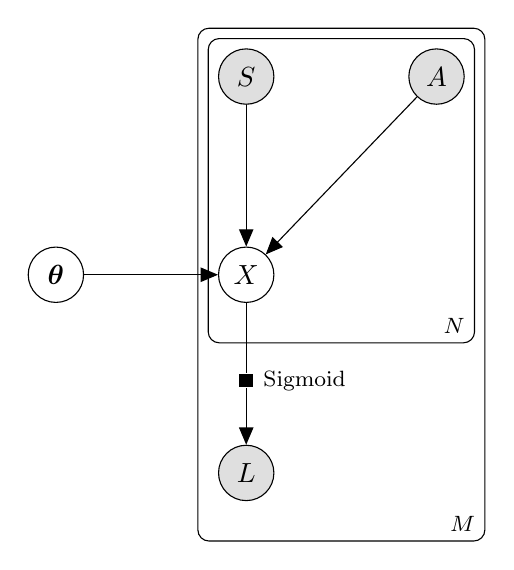
\begin{tikzpicture}[x=1.7cm,y=1.8cm]
   \node[latent]                   (R)      {$\bm{\theta}$} ; %
   \node[latent, right=of R]                   (X)      {$X$} ; %
   \node[obs, below=of X]                      (L)      {$L$} ; %
   \node[obs, above=of X]          (S)      {$S$} ; %
   \node[obs, right=of S]          (A)      {$A$} ; %
   
   \factor[above=of L]{L-f}{right:Sigmoid}{}{} ;

  \edge {S}{X} ;
  \edge {A}{X} ;
  \edge {R}{X} ;
  \factoredge {X}{L-f}{L} ;

   \plate {traj}{
   		(S) (A) (X)
   } {$N$} ;%

   \plate {data}{
   		(traj)(L-f)(L)
   } {$M$} ;

\end{tikzpicture}
\caption{Generalized IRL}
\label{fig:girl}
\end{wrapfigure}

Others are also attempting to solve similar problems~\cite{burchfiel2016distance,shiarlis2016inverse}, 
but our problem formulation, which is quite general, is also novel.
%
The plate diagram that describes this formulation is shown
in Figure~\ref{fig:girl}.  In this model, we interpret the label ($L$)
associated with a trajectory of size $N$ to be some random function of
what the evaluator thought about each of the action selections ($A$)
exhibited at each of the states ($S$) in the trajectory.  However,
these step-wise evaluations ($X$) are unobserved in the data.

For illustrative purposes, we adopt the probabilistic maximum
likelihood problem formulation, in which we seek a utility function
that maximizes the likelihood of the data, but Bayesian reasoning also
applies.
% could likewise be applied here.
%
To find the utility function that maximizes the likelihood of the data,
we first define a generative probability model for the system that is represented
in Figure~\ref{fig:girl}.
%
We model the probability that an action is evaluated as good or not as
proportional to its selection probability according a softmax policy
computed for the utility function with parameters
$\bm{\theta}$, specifically,
\comment{
\begin{align}
\Pr(x_i = +1 \mid s, a, \theta) &= \pi(s, a \mid \bm{\theta}) \\
\Pr(x_i = -1 \mid s, a, \theta) &= 1 - \pi(s, a \mid \bm{\theta}),
\end{align}
}
$\Pr(x_i = +1 \mid s, a, \theta) = \pi(s, a \mid \bm{\theta})$ and
$\Pr(x_i = -1 \mid s, a, \theta) = 1 - \pi(s, a \mid \bm{\theta})$.
%
%\noindent
Here, $\pi(s, a \mid \bm{\theta})$ is the softmax policy over $Q$-values,
assuming a utility function parameterized by $\bm{\theta}$.

\comment{
%%% DELETED B/C OF SPACE CONSTRAINTS !!!
\begin{equation}
\pi(s, a \mid \bm{\theta}) = \frac{e^{\beta Q(s,a \mid \bm{\theta})}}{\sum_{a'}e^{\beta Q(s,a' \mid \bm{\theta})}},
\end{equation}

\noindent
$\beta$ is a selectable parameter, and $Q(s,a \mid \bm{\theta})$ is the
$Q$-value computed for the utility function parameterized by
$\bm{\theta}$.
}

For the probability distribution of $L$, given the sequence of $N$
step-wise labels, we would like a distribution that has the property
that as more step-wise labels are positive, the probability of a
positive trajectory label increases (and vice versa). Although there
are many possible distributions that satisfy this property, for
concreteness, we choose the sigmoid function. That is,
%
\comment{
\begin{align}
\Pr(L = +1 \mid X_1, ..., X_n) &= \frac{1}{1 + e^{-\phi \sum_i^N X_i}} \\
\Pr(L = -1 \mid X_1, ... ,X_n) &= 1 - \Pr(L = +1 \mid X_1, ..., X_n),
\end{align}
}
$\Pr(L = +1 \mid X_1, ..., X_n) = (1 + e^{-\phi \sum_i^N X_i})^{-1}$ and
$\Pr(L = -1 \mid X_1, ... ,X_n) = 1 - \Pr(L = +1 \mid X_1, ..., X_n)$.
%
%\noindent
Here, $\phi$ is a parameter that controls how readily step-wise labels
influence the trajectory labels.  For example, when $\phi = 0$,
trajectory labels are assigned uniformly at random, without any regard
for of step-wise labels.  As $\phi \rightarrow \infty$, the sigmoid
converges to a step function in which a trajectory containing even one
more positive step-wise label than negative will deterministically
lead to a positive trajectory label (and vice versa).


%%%
\vspace{\up}
\paragraph{EM Algorithm}

The problem with estimating the parameters ($\bm{\theta}$) of a
utility function in this setting is that there is a latent variable
vector $X$ (or rather, some of the elements of the $X$ vector are
latent, and some may be observed), which makes it difficult to compute
the likelihood of the model and maximize its parameters.  The EM
approach to solving this problem is to first choose values for
$\bm{\theta}$; then choose a new $\bm{\theta}$ that maximizes the
expected value of the log likelihood function, where the distribution
in the expectation is the probability of the latent variables (the
$X$s in our case), given the observed data and previous choice of
$\bm{\theta}$.  The maximization can be performed using gradient
ascent, and this process repeats until convergence.

To simplify the exposition of the EM algorithm, we introduce the
notation $\bm{x}_k$ to indicate the values of the subset of observed
(i.e., known) elements in an $\bm{x}$ vector, and $\bm{x}_u$ to
represent a possible assignment to the subset of unobserved values.
Using this notation, the EM algorithm is summarized in
Algorithm~\ref{alg:em}.

\begin{algorithm}
\caption{EM Algorithm for GIRL}
\begin{algorithmic}
\Require{initial $\bm{\theta}^0$, and data $\bm{s}, \bm{a}, \bm{x}_k, l$}
\For{$t=0$ to $T$}
\State $\bm{\theta}_{t+1} \gets \arg \max_{\bm{\theta'}} \E_{\bm{x}_u \sim \Pr(\bm{x}_u \mid l, \bm{x}_k, \bm{s}, \bm{a}, \bm{\theta})} \left[ \log\mathcal{L}(\bm{s}, \bm{a}, \bm{\theta}' \mid l, \bm{x}) \right]$
\EndFor
\end{algorithmic}
\label{alg:em}
\end{algorithm}

The log likelihood given our plate diagram (i.e., the joint likelihood
of the data and our parameters, given label $l$ and a vector $\bm{x}$)
is
%
\comment{
\begin{align}
\Pr(l, \bm{x} \mid \bm{s}, \bm{a}, \bm{\theta}) 
&= \mathcal{L}(\bm{s}, \bm{a}, \bm{\theta} \mid l, \bm{x}) \Pr(l, \bm{x}).
\end{align}
}
%
\begin{align}
\mathcal{L}(\bm{s}, \bm{a}, \bm{\theta} \mid l, \bm{x}) 
= \Pr(l \mid \bm{x}) \prod_i \Pr(x_i \mid s_i, a_i, \bm{\theta}).
\end{align}

\noindent
Likewise, the log likelihood is
%
\begin{align}
\log\mathcal{L}(\bm{s}, \bm{a}, \bm{\theta} \mid l, \bm{x}) = 
\log \Pr(l \mid \bm{x}) + \sum_i \log \Pr(x_i \mid s_i, a_i, \bm{\theta}).
\end{align}
%
\noindent
Additionally, the gradient of the log likelihood is
%
\begin{align}
\nabla_{\bm{\theta}} \log\mathcal{L}(\bm{s}, \bm{a}, \bm{\theta} \mid l, \bm{x}) = \sum_i  \frac{\nabla_{\bm{\theta}} \Pr(x_i \mid s_i, a_i, \bm{\theta})}{\Pr(x_i \mid s_i, a_i, \bm{\theta})}.
\end{align}
%
This gradient forms the basis for the maximization step in EM.
 
The expectation in our EM algorithm is the expected value of the log
likelihood under some candidate parameter $\bm{\theta}'$, assuming
unknown values are distributed according to $\bm{\theta}$, is:
%
\begin{align*}
\E_{\bm{x}_u \sim \Pr(\bm{x}_u \mid l, \bm{x}_k, \bm{s}, \bm{a}, \bm{\theta})} \left[ \log\mathcal{L}(\bm{s}, \bm{a}, \bm{\theta}' \mid l, \bm{x}) \right]
= \sum_{\bm{x}_u} \Pr(\bm{x}_u \mid l, \bm{x}_k, \bm{s}, \bm{a}, \bm{\theta}) \log\mathcal{L}(\bm{s}, \bm{a}, \bm{\theta}' \mid l, \bm{x}_k, \bm{x}_u).
\end{align*}
%
To compute this expectation, we need to enumerate each of the
possible assignments to $\bm{x}_u$, and compute their probabilities,
given the observed data and model parameters $\bm{\theta}$.  This
probability is defined as follows:
%
\begin{align*}
\Pr(\bm{x}_u \mid l, \bm{x}_k, \bm{s}, \bm{a}, \bm{\theta}) &= \frac{\Pr(l \mid \bm{x}_k, \bm{x}_u) \Pr(\bm{x}_u \mid \bm{s}, \bm{a}, \bm{\theta}) \Pr(\bm{x}_k \mid \bm{s}, \bm{a}, \bm{\theta}) \Pr(\bm{s}, \bm{a}, \bm{\theta})}{\Pr(l \mid \bm{x}_k, \bm{s}, \bm{a}, \bm{\theta}) \Pr(\bm{x}_k \mid \bm{s}, \bm{a}, \bm{\theta}) \Pr(\bm{s}, \bm{a}, \bm{\theta})} \\
&= \frac{\Pr(l \mid \bm{x}_k, \bm{x}_u) \Pr(\bm{x}_u \mid \bm{s}, \bm{a}, \bm{\theta}) }{\Pr(l \mid \bm{x}_k, \bm{s}, \bm{a}, \bm{\theta})} \\
&= \frac{\Pr(l \mid \bm{x}_k, \bm{x}_u) \prod_i \Pr(\bm{x}_{u,i} \mid s_i, a_i, \bm{\theta}) }{\Pr(l \mid \bm{x}_k, \bm{s}, \bm{a}, \bm{\theta})}. 
\end{align*}

Unfortunately, 
%even with an efficient means to compute
%$\Pr(l \mid \bm{x}_k, \bm{s}, \bm{a}, \bm{\theta})$, 
the number of assignments enumerated in the expectation's outer sum
grows exponentially, and the product series in the above equation
($\prod_i \Pr(\bm{x}_{u,i} \mid s_i, a_i, \bm{\theta})$) can have
underflow issues.  A resolution to this first problem is to estimate
the expectation with sampling.  However
%Monte Carlo sampling is unfortunately intractable because 
it is not easy to sample from $\Pr(\bm{x}_u \mid l, \bm{x}_k, \bm{s}, 
\bm{a}, \bm{\theta})$; moreover, doing so would not address the
underflow issue in the product series.  On the other hand, it is easy
to sample from $\Pr(\bm{x}_u \mid \bm{s}, \bm{a}, \bm{\theta})$
(removing the conditioning on the label).
%
%\begin{align*}
%E_{\bm{x}_u \sim \Pr(\bm{x}_u \mid l, \bm{x}_k, \bm{s}, \bm{a}, \bm{\theta})} \left[ \log\mathcal{L}(\bm{s}, \bm{a}, \bm{\theta}' \mid l, \bm{x}) \right]
%&= \sum_{\bm{x}_u} \Pr(\bm{x}_u \mid l, \bm{x}_k, \bm{s}, \bm{a}, \bm{\theta}) \log\mathcal{L}(\bm{s}, \bm{a}, \bm{\theta}' \mid l, \bm{x}_k, \bm{x}_u) \\
%&= \sum_{\bm{x}_u} \left( \frac{\Pr(\bm{x}_u \mid l, \bm{x}_k, \bm{s}, \bm{a}, \bm{\theta})}{\Pr(\bm{x}_u^j \mid \bm{s}, \bm{a}, \bm{\theta})}\right) {\Pr(\bm{x}_u^j \mid \bm{s}, \bm{a}, \bm{\theta})} \log\mathcal{L}(\bm{s}, \bm{a}, \bm{\theta}' \mid l, \bm{x}_k, \bm{x}_u)
%\end{align*}
%
So, using importance sampling, we replace the expectation computation
with the sample-estimate
\begin{equation}
\frac{1}{C} \sum_{j=1}^C \frac{\Pr(\bm{x}_u^j \mid l, \bm{x}_k, \bm{s}, \bm{a}, \bm{\theta})}{\Pr(\bm{x}_u^j \mid \bm{s}, \bm{a}, \bm{\theta})} \log\mathcal{L}(l, \bm{x}_k, \bm{x}_u^j \mid \bm{s}, \bm{a}, \bm{\theta}).
\end{equation}
where $\bm{x}_u^j$ is the $j$th sample from the distribution $\Pr(\bm{x}_u \mid \bm{s}, \bm{a}, \bm{\theta})$.

Note that this simplifies a bit further too:
\begin{equation*}
\frac{\Pr(\bm{x}_u^j \mid l, \bm{x}_k, \bm{s}, \bm{a}, \bm{\theta})}{\Pr(\bm{x}_u^j \mid \bm{s}, \bm{a}, \bm{\theta})} 
= \left( \frac{\Pr(l \mid \bm{x}_k, \bm{x}_u) \Pr(\bm{x}_u^j \mid \bm{s}, \bm{a}, \bm{\theta}) }{\Pr(l \mid \bm{x}_k, \bm{s}, \bm{a}, \bm{\theta})} \right) \left( \frac{1}{\Pr(\bm{x}_u^j \mid \bm{s}, \bm{a}, \bm{\theta})} \right)
= \frac{\Pr(l \mid \bm{x}_k, \bm{x}_u)}{\Pr(l \mid \bm{x}_k, \bm{s}, \bm{a}, \bm{\theta})}
\end{equation*}

\noindent
Consequently, we have removed the product series from the expectation
weight, thereby avoiding underflow issues. Also, while a
straightforward computation of
$\Pr(l \mid \bm{x}_k, \bm{s}, \bm{a}, \bm{\theta})$ requires
marginalizing over all possible assignments to $\bm{x}_u$, this term
can be actually computed efficiently using dynamic programming,
because the probability of a label is a sigmoid function that operates
on the \emph{sum\/} of the entries in the $\bm{x}$ vector.

Putting all of these pieces together yields a tractable version of the
EM algorithm for generalized IRL (Algorithm~\ref{alg:tractable}).

%%% DELETED B/C OF SPACE CONSTRAINTS !!!
\begin{algorithm}
\caption{Approximate EM Gradient Ascent Algorithm}
\begin{algorithmic}
\Require{initial $\bm{\theta}_0$; data $\bm{s}$, $\bm{a}$, $\bm{x}_k$, $l$; and learning rate $\alpha$}
\For{$t=0$ to $T$}
\State draw $j=1$ to $C$ samples of $\bm{x}_u^j \sim \Pr(\bm{x}_u \mid \bm{s}, \bm{a}, \bm{\theta}_t)$ 
\For{$j=1$ to $C$}
\State $w_j \gets \frac{\Pr(l \mid \bm{x}_k, \bm{x}_u)}{\Pr(l \mid \bm{x}_k, \bm{s}, \bm{a}, \bm{\theta}_t)}$ \Comment{Expectation step}
\EndFor
\State $\bm{\theta}' \gets \bm{\theta}_t$
\For{1 to $M$} \Comment{Gradient ascent maximization loop}
\State $\bm{\theta}' \gets \bm{\theta}' + \alpha \frac{1}{C} \sum_{j=1}^C w_j \left( \sum_{x_i \in \bm{x}_k \cup \bm{x}_u^j} \frac{\nabla_{\bm{\theta}'} \Pr(x_i \mid s_i, a_i, \bm{\theta}')}{\Pr(x_i \mid s_i, a_i, \bm{\theta}')} \right)$
\EndFor
\State $\bm{\theta}_{t+1} \gets \bm{\theta}'$
\EndFor
\end{algorithmic}
\label{alg:tractable}
\end{algorithm}



\vspace{\up}
\paragraph{EM Algorithm}

The problem with estimating the parameters ($\bm{\theta}$) of a
utility function in this setting is that there is a latent variable
vector $X$ (or rather, some of the elements of the $X$ vector are
latent, and some may be observed), which makes it difficult to compute
the likelihood of the model and maximize its parameters.  The EM
approach to solving this problem is to first choose values for
$\bm{\theta}$; then choose a new $\bm{\theta}$ that maximizes the
expected value of the log likelihood function, where the distribution
in the expectation is the probability of the latent variables (the
$X$s in our case), given the observed data and previous choice of
$\bm{\theta}$.  The maximization can be performed using gradient
ascent, and this process repeats until convergence.

To simplify the exposition of the EM algorithm, we introduce the
notation $\bm{x}_k$ to indicate the values of the subset of observed
(i.e., known) elements in an $\bm{x}$ vector, and $\bm{x}_u$ to
represent a possible assignment to the subset of unobserved values.
Using this notation, the EM algorithm, at a high level, is summarized
in Algorithm~\ref{alg:em}.
%
We have derived a dynamic programming algorithm that, coupled with
importance sampling, yields a tractable version of EM for the
generalized IRL problem.

\begin{algorithm}
\caption{EM Algorithm for GIRL}
\begin{algorithmic}
\Require{initial $\bm{\theta}^0$, and data $\bm{s}, \bm{a}, \bm{x}_k, l$}
\For{$t=0$ to $T$}
\State $\bm{\theta}_{t+1} \gets \arg \max_{\bm{\theta'}} \E_{\bm{x}_u \sim \Pr(\bm{x}_u \mid l, \bm{x}_k, \bm{s}, \bm{a}, \bm{\theta})} \left[ \log\mathcal{L}(\bm{s}, \bm{a}, \bm{\theta}' \mid l, \bm{x}) \right]$
\EndFor
\end{algorithmic}
\label{alg:em}
\end{algorithm}


%
\section{DP Algorithm For Label Probability}

One of the terms that must be computed for the EM algorithm weight is $\Pr(l \mid \bm{x}_k, \bm{s}, \bm{a}, \bm{\theta})$. A straightforward computation of this value would involve marginalizing over $\bm{x}_u$, which grows exponentially large as the number of unknown feedbacks increases. However, by exploiting the fact that $\Pr(l | \bm{x}_k, \bm{x}_u, \bm{s}, \bm{a}, \bm{\theta})$ is a function of the sum of the feedback values, the marginalization can be reduced to a summation that iterates over a number of values that is a linear function of the number of unobserved feedbacks. To demonstrate, first note that $\Pr(l \mid \bm{x}, \bm{s}, \bm{a}, \bm{\theta})$, where all feedback values are known, is defined as
\begin{equation}
\Pr(l \mid \bm{x}, \bm{s}, \bm{a}, \bm{\theta}) = S\left(\sum_{x \in \bm{x}} x \right),
\end{equation} 
where $S$ is the sigmoid function. Therefore, $\Pr(l \mid \bm{x}_k, \bm{s}, \bm{a}, \bm{\theta})$, where some of the feedbacks are unobserved, can expressed by marginalizing over the possible {\em sums} of the unknown feedbacks, rather than marginalizing over all possible feedback assignments:
\begin{equation}
\Pr(l \mid \bm{x}_k, \bm{s}, \bm{a}, \bm{\theta}) = \sum_{\tau = -|\bm{x}_u|}^{|\bm{x}_u|} S\left(\tau + \sum_{x \in \bm{x}_k} x\right) \Pr(\tau \mid \bm{s}_u, \bm{a}_u, \bm{\theta}),
\end{equation}
where $\Pr(\tau \mid \bm{s}_u, \bm{a}_u, \bm{\theta})$ is the probability that the unknown feedbacks will sum to $\tau$, given the states and actions for the unknown feedbacks, and the model parameters $\bm{\theta}$.

Computing this simpler marginal distribution requires computing $\Pr(\tau \mid \bm{s}_u, \bm{a}_u, \bm{\theta})$: the probability distribution of the sum of possible feedback values. Fortunately, this probability can expressed recursively and computed efficiently with a dynamic programming algorithm. 

To describe this recursive relationship, note that if we knew the probability distribution of the sum of feedback values for all unknown feedbacks except the last of them, then we could compute the probability that {\em all} of the feedbacks would some to some value $\tau$ as the probability that the remaining feedbacks sum to $\tau - 1$ and the last feedback is a $+1$ {\em or} the remaining feedbacks sum to $\tau + 1$ and the last feedback is a $-1$. That is,
\begin{align}
\Pr(\tau_n = \tau \mid \bm{s}_n, \bm{a}_n, \bm{\theta}) =& \Pr(x_n = +1 \mid s_n, a_n) \Pr(\tau_{n-1} = \tau_n - 1 \mid \bm{s}_{n-1}, \bm{a}_{n-1}, \bm{\theta}) \nonumber \\
& + \Pr(x_n = -1 \mid s_n, a_n) \Pr(\tau_{n-1} = \tau_n + 1 \mid \bm{s}_{n-1}, \bm{a}_{n-1}, \bm{\theta}), 
\end{align}
where $n$ is the number unobserved feedbacks, $\tau_i$ is the random variable specifying the sum of the first $i$ unobserved feedbacks; $s_i$ and $a_i$ represents the $i$th state and action that are associated with unobserved feedback $x_i$; $\bm{s}_i$, $\bm{a}_i$ represents the set of the first $i$ state and actions associated with the unobserved feedbacks; and finally, where the probability of the first unobserved feedback summing to $\tau$ is defined as the probability that the first feedback takes that value:
\begin{equation}
\Pr(\tau_1 = \tau \mid \bm{s}_n, \bm{a}_n, \bm{\theta}) = \begin{cases}
\Pr(x_n = +1 \mid s_n, a_n) & \mbox{if } \tau_1 = 1 \\
\Pr(x_n = -1 \mid s_n, a_n) & \mbox{if } \tau_1 = -1 \\
0 & \mbox{otherwise}
\end{cases}.
\end{equation}
We can compute this recursive probability distribution using dynamic programming in which we build a $2n+1 \times n$ matrix, where cell $i,j$ specifies the value for $\Pr(\tau_j = i \mid \bm{s}_j, \bm{a}_j, \bm{\theta})$. The values for the matrix are then filled out column by column, from $j=1$ to $n$. Consequently, using this DP algorithm, we can compute the $\Pr(l \mid \bm{x}_k, \bm{s}, \bm{a}, \bm{\theta})$ term required for our EM weight in only $O(|\bm{x_u}|^2)$ time, rather than $O(2^{|\bm{x_u}|})$.


%\begin{figure}
\begin{minipage}{0.2\textwidth}
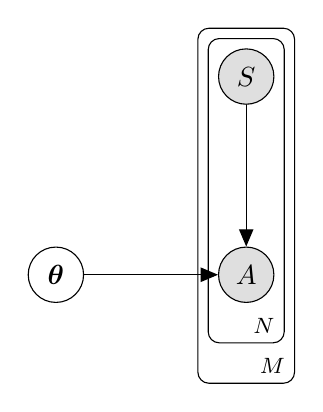
\begin{tikzpicture}[x=1.7cm,y=1.8cm]
   \node[latent]                   (R)      {$\bm{\theta}$} ; %
   \node[obs, right=of R]                   (X)      {$A$} ; %
   \node[obs, above=of X]          (S)      {$S$} ; %
   

  \edge {S}{X} ;
  \edge {R}{X} ;

   \plate {traj}{
      (S) (X)
   } {$N$} ;%

   \plate {data}{
      (traj)
   } {$M$} ;

\end{tikzpicture}
\captionof{figure}{Classic IRL}
\label{fig:irl-plate}
\end{minipage}%
%
\hspace{0.04\textwidth}
\begin{minipage}{0.205\textwidth}
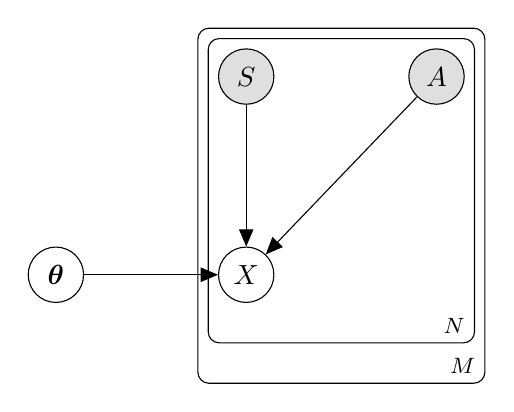
\begin{tikzpicture}[x=1.7cm,y=1.8cm]
   \node[latent]                   (R)      {$\bm{\theta}$} ; %
   \node[latent, right=of R]                   (X)      {$X$} ; %
   \node[obs, above=of X]          (S)      {$S$} ; %
   \node[obs, right=of S]          (A)      {$A$} ; %
   

  \edge {S}{X} ;
  \edge {A}{X} ;
  \edge {R}{X} ;

   \plate {traj}{
      (S) (A) (X)
   } {$N$} ;%

   \plate {data}{
      (traj)
   } {$M$} ;

\end{tikzpicture}
\captionof{figure}{SABL Label}
\label{fig:sabl}
\end{minipage}%
%
\hspace{0.175\textwidth}
\begin{minipage}{0.22\textwidth}
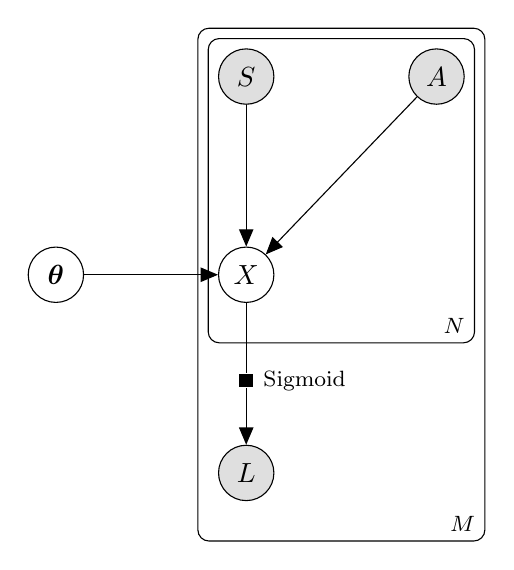
\begin{tikzpicture}[x=1.7cm,y=1.8cm]
   \node[latent]                   (R)      {$\bm{\theta}$} ; %
   \node[latent, right=of R]                   (X)      {$X$} ; %
   \node[obs, below=of X]                      (L)      {$L$} ; %
   \node[obs, above=of X]          (S)      {$S$} ; %
   \node[obs, right=of S]          (A)      {$A$} ; %
   
   \factor[above=of L]{L-f}{right:Sigmoid}{}{} ;

  \edge {S}{X} ;
  \edge {A}{X} ;
  \edge {R}{X} ;
  \factoredge {X}{L-f}{L} ;

   \plate {traj}{
   		(S) (A) (X)
   } {$N$} ;%

   \plate {data}{
   		(traj)(L-f)(L)
   } {$M$} ;

\end{tikzpicture}
\captionof{figure}{Feedback IRL}
\label{fig:feedback}
\end{minipage}
\end{figure}


\vspace{\up}
\paragraph{Preliminary Experiments}

We ran some (very) preliminary experiments to demonstrate the
potential of our EM approach in the GIRL framework.%
%\footnote{A description of the algorithm was omitted because of space constraints.}
\footnote{Because the problem domain in these experiments
was small (a 5 $\times$ 5 grid), we did not need importance sampling.}
%
The agent is operating in a grid world (see
Figure~\ref{fig:puddle-grid}), with puddles of multiple colors: red,
blue, green, yellow and pink.  The agent (gray circle) can take north, south, east
and west actions.
%If there is a wall in the way, the agent does not move at all.
%For example if the agent tries to move east and it is next to the eastern wall of the grid, it doesn't move at all.  
In these experiments, we gave the agent two very short
trajectories, and a corresponding pair of positive and negative
labels.  We show that varying these labels leads the agent to
infer different utility functions, and correspondingly different
behaviors.

In both trajectories, the agent begins in the middle cell of the
bottom row of the grid (as shown).  The first trajectory has the agent
move two steps to the west, through the blue puddle, and terminating
at the red puddle.  The second trajectory has the agent move a single
step west, terminating at the blue puddle.
%
%These trajectories are shown in the first set of Figures~\ref{fig:trajectories}.
%
We compare three different labelings for these trajectories (all three
labelings that include at least one positive label): two positive
($+1$ for each), positive \& negative ($+1$ for first, $-1$ for
second), and negative \& positive ($-1$ for first, $+1$ for
second). The learned policies, along with shading that reflects
inferred utility values (blue is high; red is low; and shades of
purple, in between)
%(along with corresponding, but illegible, rewards)
are shown in Figures~\ref{fig:test1},~\ref{fig:test2},
and~\ref{fig:test3}, respectively.

The two positive labels signal to the agent that both observed
behaviors are good.  Consequently, the agent infers that the red
puddle is worth more than any other cell in the grid and seeks
shortest paths for reaching it.  Note that the agent does not learn to
linger on the blue puddle, or direct its attention toward any other
blue puddles in the grid---even though one trajectory ended
there---because both trajectories have positive labels, and ultimately
lead to the red puddle.

Given positive \& negative labels, the agent again infers that
reaching the red puddle is good and the blue puddle is not good. In
contrast to the previous case, however, it infers that all other cells
are also good. This example illustrates the power of our model to
learn from negative examples. By asserting that the path terminating
at the blue puddle is bad, the agent infers that the correct path for
reaching the red puddle must be to go around the blue puddle.
% zzz these colors are almost maximally confusing. red turns blue and
% zzz blue turns red. yellow and green would have been preferable.
% zzz also, it would have been more interesting to have a negative
% label on a two-step path as the learner has to figure out which step
% was bad.
%As in experiment 1, the red puddle has the highest value in the grid.

The agent sees negative \& positive labels as a signal that the red
puddle is to be avoided and getting to the blue puddle is good.  This
time, the agent prefers the blue puddles to the red, and it finds a
policy by which it can reach, and remain in, blue puddles.
%\commentm{these grids seem like overkill for the point we're able to make. Ah, well.}
%\commenta{agreed, totally!}

In a fourth experiment (not shown), we labelled both trajectories
$-1$.  Given this information, the agent learns to avoid all puddles,
and directs all its movements towards the white spaces on the grid,
instead.

These experiments demonstrate an approach to GIRL, in which agents
learn utility functions from both positive and negative examples.
% We expect this capability to prove essential for humans hoping to teach agents to collaborate.  
We plan to further hone this and related approaches, so that we can
eventually bring them to bear in the context of interactive learning
of social utility functions, thereby enabling artificial agents to
learn from rich human evaluative feedback.

\comment{
Beyond what is possible now, generalized IRL algorithms will allow us,
the humans, to critique agents during our interactions with them,
ascribing to their behaviors 
%(entire trajectories and subtrajectories)
both positive and negative feedback. Based on this feedback, the
agents will infer social utility functions, which we expect to
generalize well, certainly within the domain in which they train, and
with some effort, across learning environments.
}

\begin{figure}
\centering
\begin{minipage}{0.25\textwidth}
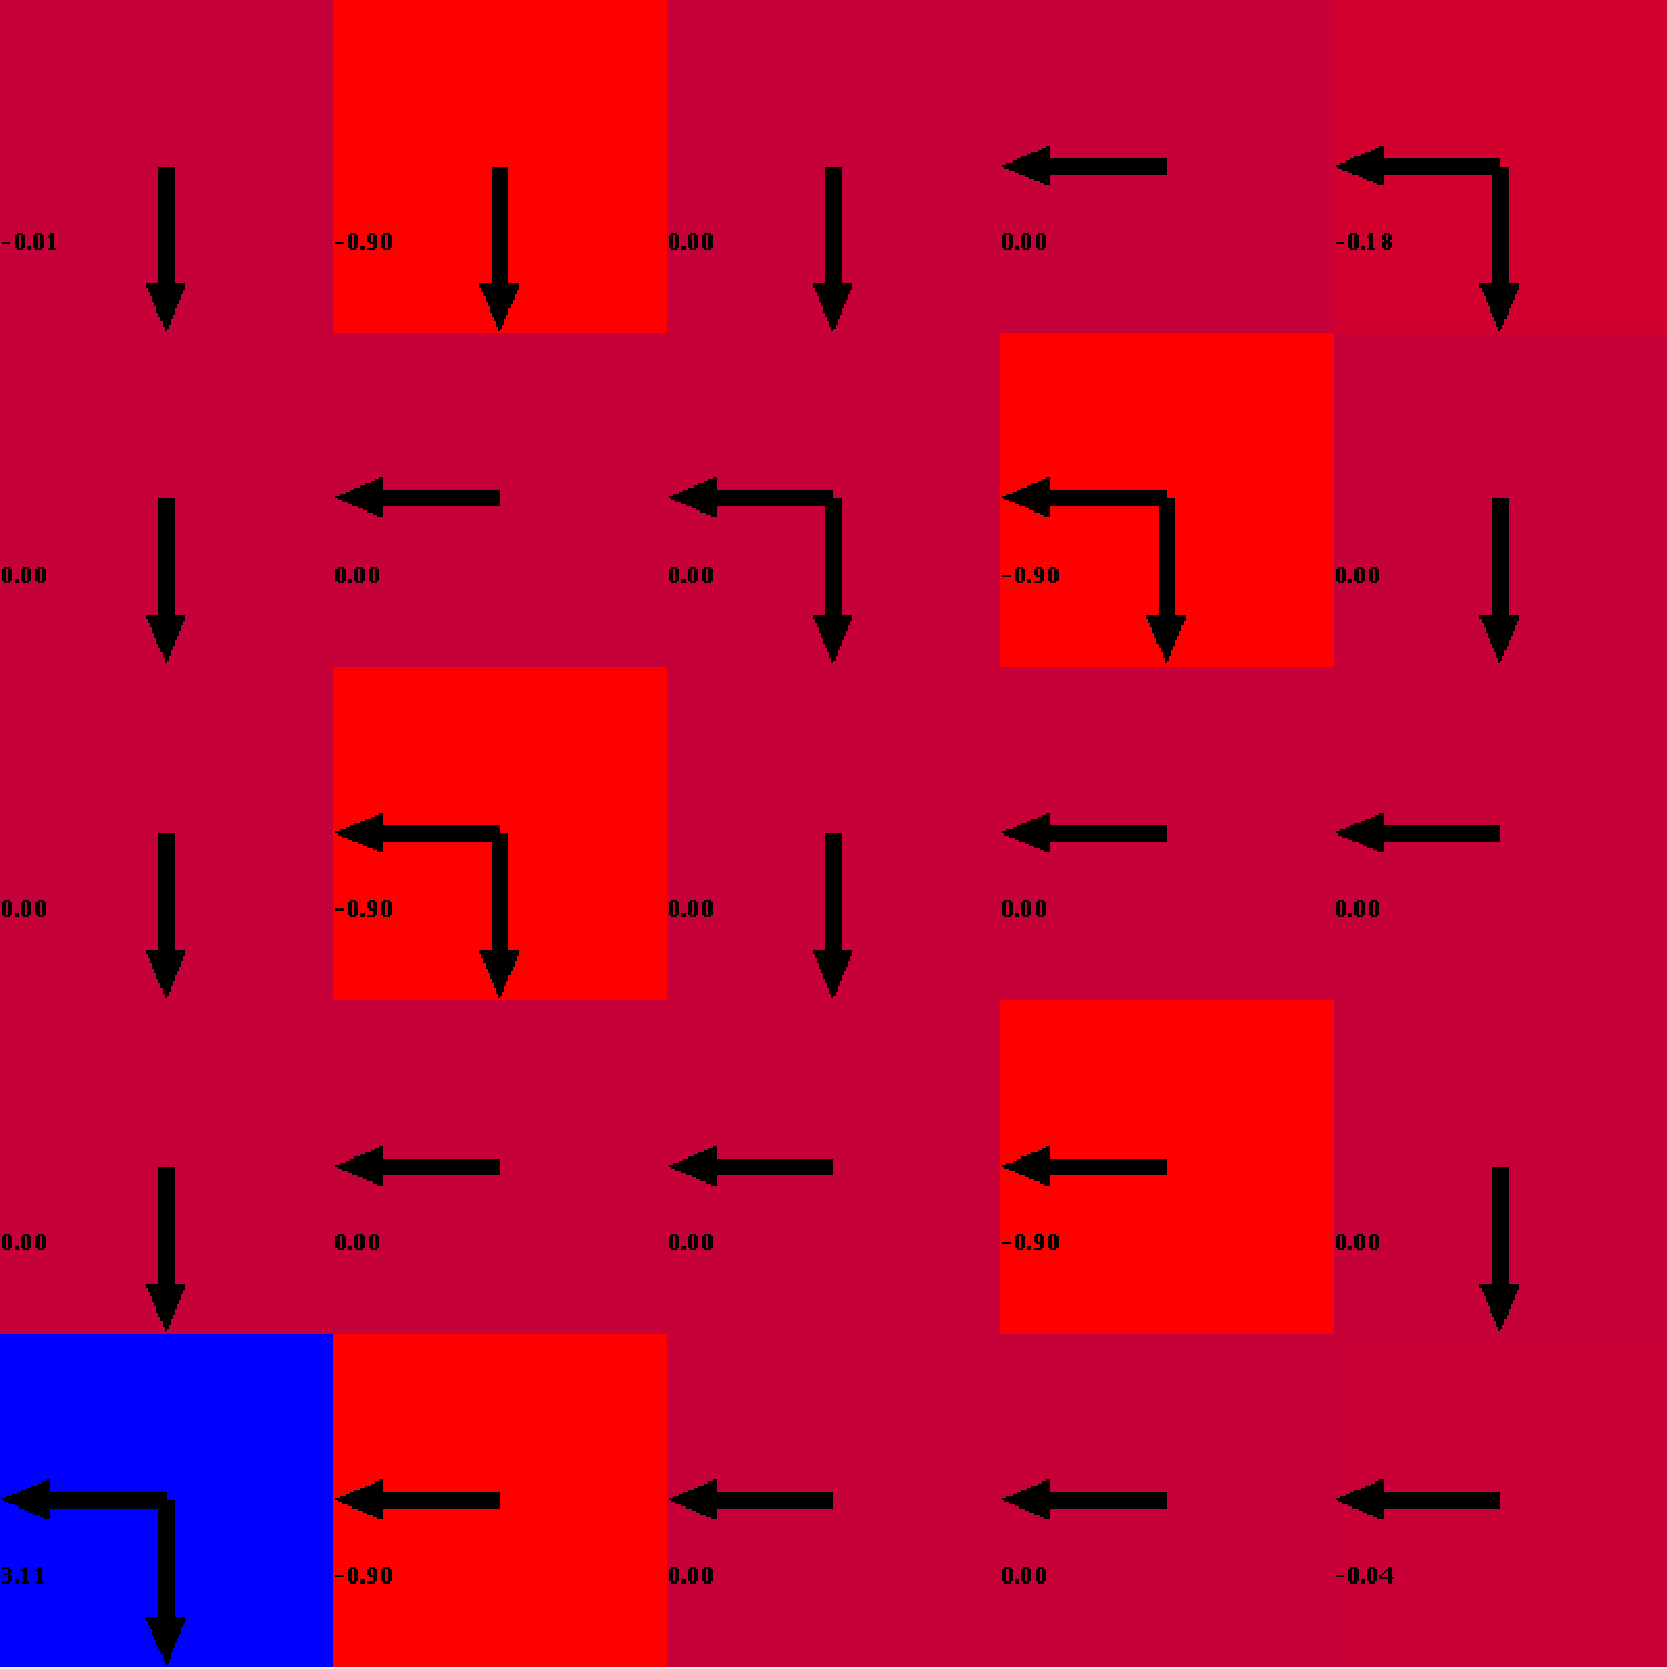
\includegraphics[width=1\columnwidth]{../2015_grant/figures/plus1plus1.pdf}
\captionof{figure}{Two positive labelled trajectories.}
\label{fig:test1}
\end{minipage}%
%
\hspace{0.04\textwidth}
%
\begin{minipage}{0.25\textwidth}
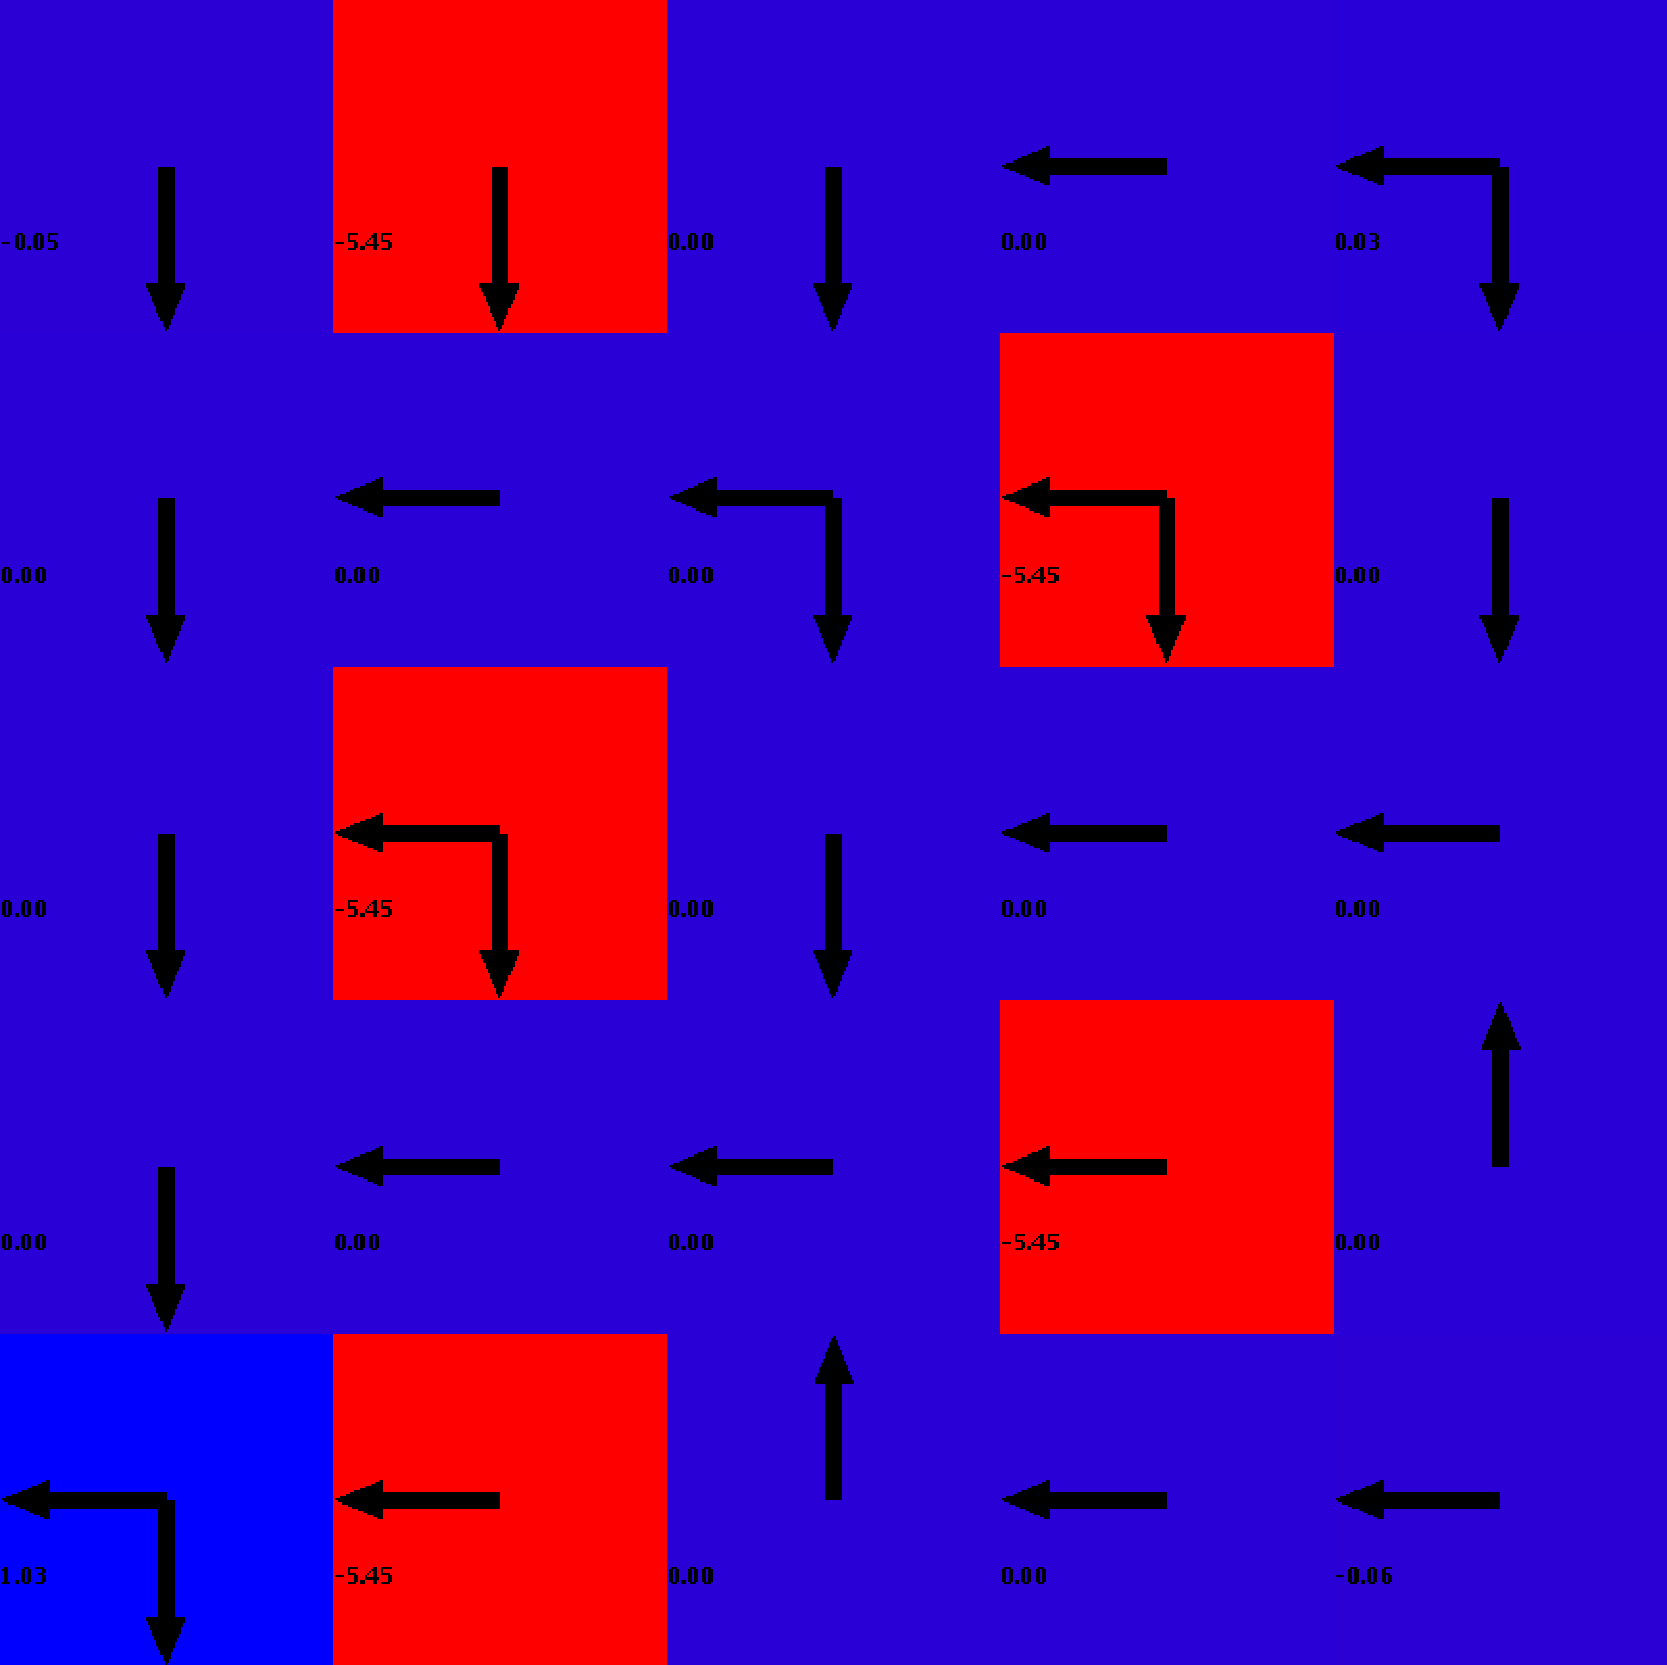
\includegraphics[width=1\columnwidth]{../2015_grant/figures/plus1minus1.pdf}
\captionof{figure}{Positive \& negative labelled trajectories.}
\label{fig:test2}
\end{minipage}%
%
\hspace{0.04\textwidth}
%
\begin{minipage}{0.25\textwidth}
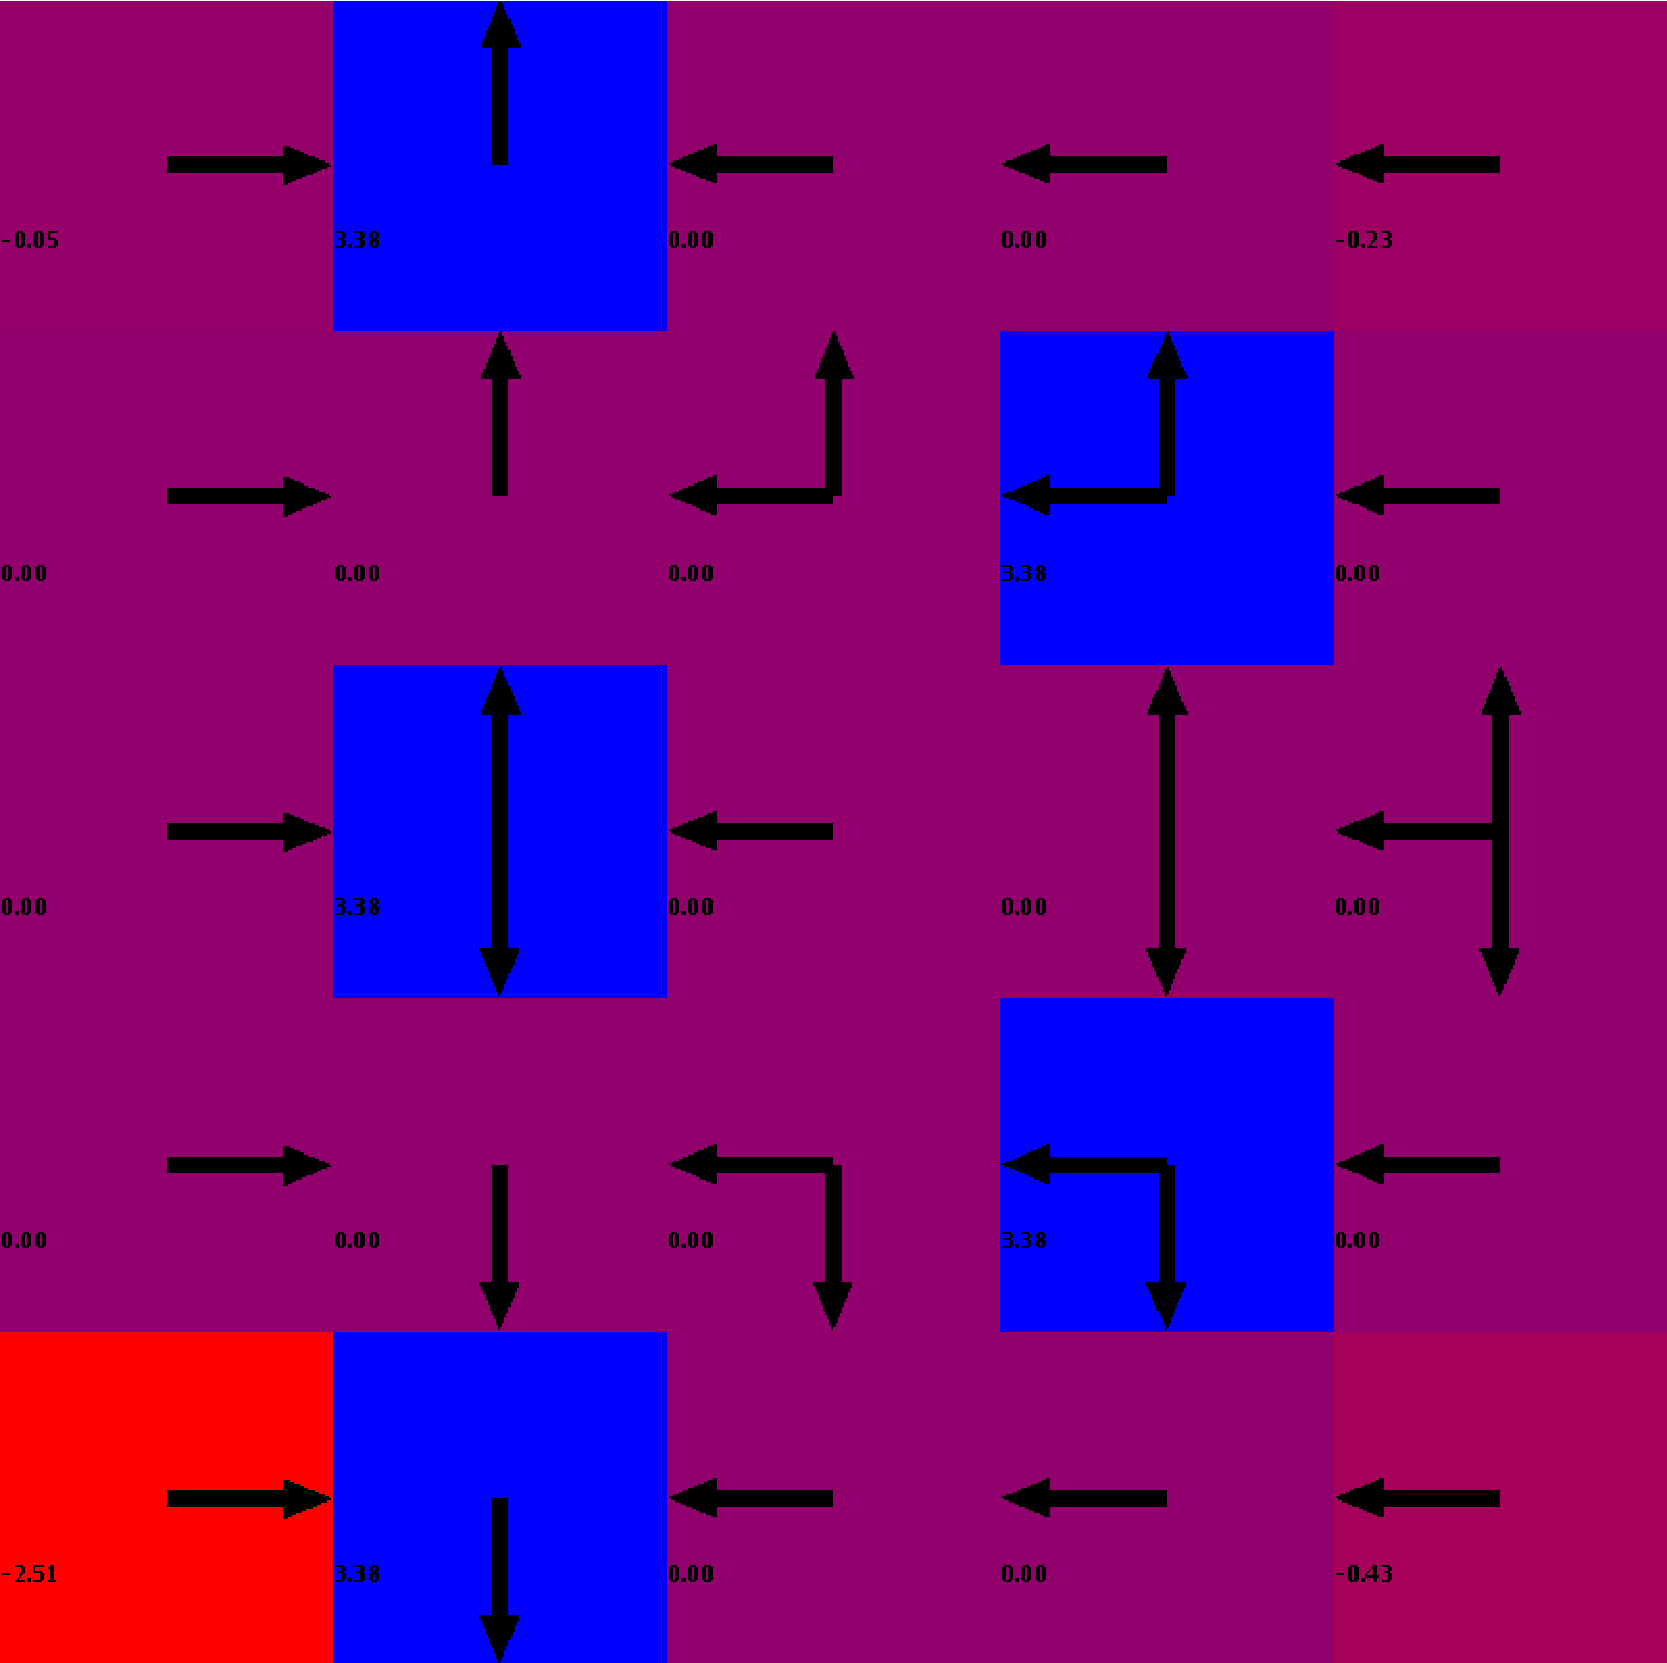
\includegraphics[width=1\columnwidth]{../2015_grant/figures/minus1plus1.pdf}
\captionof{figure}{Negative \& positive labelled trajectories.}
\label{fig:test3}
\end{minipage}
\end{figure}


% OLD
%
The algorithms described in this proposal are designed for learning
among a small set of artificial agents, usually one or two.  We will
investigate generalization across games, so that if agents learn to
play one game well, they can also play a similar game well.
%
Likewise, we expect that agents who learn to work well with one human
can also work well with another who behaves similarly.  Similar
behavior across different people in the same environment is often
described as a \mydef{social norm} (especially when there are
sanctions for not behaving as expected)~\cite{bicchieri2005grammar}.
In other words, we seek to design and build agents capable of learning
social norms.  To evaluate the norm-learning capabilities of our
agents, we will study the evolution of norms in purely human groups to
that of hybrid human-machine groups.

%One possible direction is to have the agent learn multiple norms using reward function clustering similar to that in multiple intention IRL~\cite{babes11}, and then homogenize the clusters as the various subpopulation's behaviors converge. 

%To evaluate adaptivity in populations, we will compare the results of purely human populations with human-agent populations.



% 3.5 page
\section{Plan, Deliverables, and Evaluation}

\vspace{\up}
\paragraph{Plan}

The three-year timeline for our proposed project is as follows:

\begin{itemize}
\item {\bf Year 1}: Demonstrate that a socially rational agent can
  successfully learn collaborative behavior from batches of
  demonstrations (offline), and can generalizate across related games.
  Carry out simulation experiments on machine--machine pairings,
  varying both the algorithms and the environments.  Complete the
  development of an experimental test bed that pairs humans with
  artificial agents.

\item {\bf Year 2}: Establish that IRL algorithms within the GIRL
  framework can learn more accurately and more efficiently (i.e., from
  fewer data) than classic IRL algorithms, because of the ability of
  the teacher to offer both positive and negative feedback.
  Incorporate GIRL learning algorithms into the Year 1 experimental
  test bed, and show how collaborative behavior can emerge in
  real-time during human--machine interactions.  Develop the proposed
  ``Social autonomous driving'' course (see Broader Impacts).
%   determine whether an interaction is proceeding collaboratively, 
%   or if cooperation has broken down and players should revert to 
%   more traditional self-interested behavior. 

\item {\bf Year 3}: Extend as necessary, and then evaluate our
  approach in real-world applications, specifically to the ``go
  fetch'' scenario (see Broader Impacts).
%   Algorithmically, we will focus on ways an agent can actively teach 
%   its partner to adopt mutually beneficial behavior.
%\commentm{We could propose ``deep IRL'' ... since MLIRL is a gradient method, it should be easy to incorporate it into standard deep learning packages to learn complex social utility functions.}

\end{itemize}



\section{Deliverables}

The proposed project includes the following deliverables: 

\begin{enumerate}

\item An {\em experimental platform\/} in which humans can interact
  with artificial agents, thereby providing a space for
  artificial agents to demonstrate their capacity to represent, learn,
  and apply cooperative behaviors in context-appropriate ways.

\item {\em Software infrastructure for machine learning algorithm
  development and experimentation\/} that enable the representation
  and learning of cooperative behaviors in simulated stochastic games.
  Code will be made available as a part of the Brown-UMBC
  Reinforcement Learning and Planning library.%
\footnote{The open source Brown-UMBC Reinforcement Learning and
  Planning (BURLAP) library (\url{http://burlap.cs.brown.edu}) is the
  software infrastructure that will be used for algorithm development
  in this project.  Developed by James MacGlashan under the direction
  of co-PI Littman, the system provides a flexible and powerful
  implementation of a wide variety of reinforcement-learning
  algorithms and environments, and has been extensively used in both
  published research and education (including in a
  reinforcement-learning MOOC).  The algorithm which formed the basis
  of the work we describe in this proposal (RHC-MLIRL) is available as
  part of the BURLAP distribution.}

\item Data comprised of the behaviors produced by both humans and
  machines on a test bed of stochastic games, varying the degrees of
  complexity and uncertainty, as well evaluations of those behaviors.
  It is our intent that these data will form a set of {\em
    computational benchmarks}, which other researchers will be free to
  use to evaluate their own approaches to collaborative learning.

\item Syllabus for an undergraduate class on ``Social autonomous
  driving'' in which students learn to endow autonomous driving
  vehicles with the ability to represent, learn, and apply cooperative
  driving algorithms.

\end{enumerate}

In year two, we plan to organize a workshop (e.g., a AAAI symposium)
on the machine learning of socially rational behavior. Such a
gathering would be timely, as a number of subareas are grappling with
related problems. We will include researchers in human--robot
collaboration~\cite{gopalan15}, intelligent software\commenta{missing reference}, end-user
programming of household devices~\cite{ur14}, agent-based
bidding~\cite{tac:book}, multi-agent reinforcement
learning~\cite{sodomka13}, computational social
cognition~\cite{baker14}, and others.\commenta{do you want to reference self-driving cars here?}



\vspace{\up}
\paragraph{Evaluation}

%Before scaling to embodied robots
We will evaluate how our socially rational agents fare in
collaborative learning tasks using an experimental platform that
simulates interactions between humans and artificial agents.
Specifically, we will compare how often and how quickly humans are
able to arrive at coordinated plans among themselves and compare to what happens with
socially rational agents.  We will also assess the quality of the
plans that emerge under these varying conditions.  
% To test the
% expressiveness of the space of learnable solutions afforded by our
% approach, we will also measure tendencies among humans to converge to
% certain types of plans (e.g., trading off simplicity for optimality),
% and whether those types persist when there are agents in the mix.
Subjective evaluations will be used to assess whether humans
find interacting with agents ``natural.''

For the batch-learning algorithm, we will develop new quantitative
metrics to assess behavioral similarity so that trajectories produced
by our batch learners can be quantitatively compared to trace data
produced by human participants.  Additionally, we plan to design a
sort of ``Turing test'' for our problem domain, whereby we will have
two humans interact with each other for a number of rounds and then,
without notification, we will fork those interactions into two, where
each human is now playing with a socially rational agent trained
on the history of interactions between the two humans.  At the end of
all interactions, we will probe whether the participants noticed anything
strange partway through the interactions.
% Their subjective responses about whether they thought their partner
% switched at any point will be compared across a variety of treatments,
% such as: (1)~no change; (2)~swapping their partner for a
% socially rational agent as already mentioned, and one that learned by
% observing other human--human interactions; (3)~swapping their partner
% for another human who observed the previous interactions, and one who
% is experienced at the task, but not with the given partner.

We are particularly interested in designing flexible agents that
generalize their behavior at least as well as humans do to new
environments.
%
An underlying goal, therefore, will be to engineer the underlying
structure of social utility functions so that they generalize well
across environments.  We we will start by examining standard
feature-selection methods used in existing reinforcement-learning and
IRL 
research (e.g., linear models, neural networks,
etc.)~\cite{diuk2009adaptive,kolter2009regularization,li2009reinforcement,parr2008analysis},
and build on them, as necessary. Given that MLIRL is a gradient-based
approach, we will explore the use of existing deep learning packages
to scale to richer utility functions and input spaces.
%
% We will evaluate our efforts at generalization by first having humans
% learn in one environment.  Afterwards, they will be exposed to a new
% environment where their previous behavior is no longer directly
% applicable (e.g., because a wall was inserted along the path that an
% agent would normally take), but a more ``general'' behavior can be
% transferred (e.g., I take the high road; he takes the low, regardless
% of the presence or absence of obstacles).  Then, using evaluations
% similar to those listed above, we will test whether our socially
% rational agents can generalize to new games as well as other humans
% can.

% \commenta{do we want to say something about generalizing to other players? maybe humans are better at this than our agents will be?} ML: No, I think the notion of generalizing rapidly to new users is a distinct learning problem.

In Year Three, we will test our approach in a real-world robot--human
collaboration domain.  Even if (as we expect), our simulated worlds
show that our agents collaborate well with people, the capabilities
(or lack thereof) of robots may inhibit the effectiveness of our
approach (e.g., robots might move slower than people expect and/or may
misperceive important details).  We will evaluate our algorithmic
framework in real-world scenarios by comparing its performance at
controlling a robot to another human controlling the robot via
teleoperation.  We expect this approach to raise novel research
questions appropriate to real-world problems.
%Amy: sounds too generic, i think. we always want to develop more efficient implementations, don't we?
%%For example, computation time may be a limiting factor to the success
%%of our machine agents, and if so, we will focus our efforts on
%%developing more efficient implementations.

% OLD STUFF
%
% Evaluation metrics that capture trajectory similarity across diverse
% games are key for assessing performance, and will drive the
% development of our learning algorithms towards more beneficial
% behavior.
% 
% We will also develop ways for people to also assess how natural it is
% to interact with our artificial agents. For example, we will
% investigate whether having two humans interact for awhile, and then,
% without notifying them, swapping their partner with an artificial
% agent trained from the interaction history results in a noticeable
% change in behavior. Participants would be asked if they noticed a
% change, and behavior would be compared between a variety of cases, 
% such as: no swap; or swapping in a trained agent, an untrained agent, 
% a human who witnessed the history of interactions, a human who did not.
%
% We will evaluate generalization by first having users learn in one
% grid. Afterwards, they will be exposed to a new grid where their
% previous behavior is no longer directly applicable (e.g., because a
% wall was inserted along the path that an agent would normally take),
% but a more ``general'' behavior can be transfered (e.g., I take the
% high road; he takes the low, regardless of the presence or absence of
% obstacles).


\section{Broader Impacts}

Recent trends in computer science and artificial intelligence are
moving us toward increasing dependence on human--computer
collaborative systems in which people and software make decisions that
impact one another.  Some fields, such as human--computer interaction
(HCI), focus on systems in which a human being is primarily in
control, and the computer's decisions are assessed in terms of the
positive impact they have on the user.  An interesting recent example
is Centaur
chess\footnote{\url{http://www.huffingtonpost.com/mike-cassidy/centaur-chess-shows-power_b_6383606.html}}
in which a human and machine team up to play on the same side in
chess, both making decisions, but with the machine acting as an
advisor and the human deciding which moves to actually make.  Other
fields, like crowd sourcing human computation~\cite{von2009human},
combine human and machine expertise such that the machine is the
ultimate arbiter of behavior and a group of human beings act as lower
level computational components.

True collaboration, however, does not start with one participant being
assigned to a leadership role.  Instead, the various agents need to
dynamically negotiate their roles and jockey for position, discovering
when and how to trust each other to move forward.  A concrete example
is in the context of self-driving cars.  Cars share the road with each
other and must carefully choose when to be responsive to other
vehicles and when to assert themselves to create a situation that
benefits them.  Doing so makes a significant difference in the
driving's effectiveness~\cite{cunningham2015mpdm}.  A related problem
arises when a self-driving wheelchair attempts to move through a group
of pedestrians~\cite{kim2016socially}.  More generally, robots that
interact with people in the physical world need to navigate the
complex give-and-take of establishing mutually beneficial behaviors
where possible.

Indeed, a wide variety of human--machine interaction problems would be
positively impacted by the technology we are proposing.
%
As such, the project is synergistic with Brown University's Humanity
Centered Robotics Initiative (HCRI), of which co-PI Littman is
co-director.  Specifically, within HCRI, there are ongoing efforts to
design robotic systems that interact with people and support
independent living tasks (e.g., gerontechnological support for aging
in place and robotic sous chefs).  For an elderly person (or chef) to
trust and collaborate on tasks with a machine effectively, the machine
must act in a manner that the elderly person (or chef) expects.  This
project creates the foundation for these important applications.

The most direct application of our ideas would be in scenarios in
which a robot is sharing a space with bystanders (human or robotic)
who do not necessarily share its goals---a personal grocery-store
assistant, a socially aware vacuum, an automated hospital linen cart,
a package delivery drone.  To further develop our ideas in a physical
environment like these, and moreover in embodied robots,
% in year 3, team up with George and/or Stefanie. by then, there will
% be robots in the department that can both move and move things around
we plan to build a ``go fetch'' application on a mobile-manipulation
platform that is scheduled for deployment in the Brown Computer
Science department in Spring 2017.  To be successful in this capacity,
a robot will need to be able to represent, learn, and apply
collaborative behavior in (at least) three separate spheres:
%
%\begin{itemize}
(1)~navigating smoothly through the atrium and hallways, finding
  appropriate ways to avoid collisions, and adopting regularities that
  make it easy for people to coordinate their own movements with it;
%
(2)~riding in the elevator, which brings with it some related but
  distinct expectations for coordinating (moving in and out of the
  doors, standing inside, asking for help with the buttons, deciding
  what to do when obstructed, etc.);
%
(3)~understanding how to best signal a handoff of the object it is
  fetching, by interrupting people without being too timid or too
  boorish.
%\end{itemize}

%This task, is within our technological limitations (unlike wheelchairs or actual cars) 
%and would definitely result in some impact if our algorithms were able to help.

Interest in robotics and machine learning is growing within the Brown
CS department.  Presently, our faculty is designing a new robotics
introductory course sequence that includes classes on basic robotics
algorithms, hardware design, and human-centered evaluation of robotics
systems.  Inspired by the ideas in this proposal, we plan to
contribute to this effort a new intermediate robotics course for
undergraduates called ``Social autonomous driving.''  As a test
platform, we will use MIT's Duckietown
platform\footnote{\url{http://duckietown.mit.edu/}, which we have installed at Brown}.
Using this platform as a test environment, students will
develop robotic drivers.  The main emphasis will be on making sure
those drivers interact smoothly with other robotic and
remote-controlled cars.  The latter will be achieved by endowing the
robots with socially rational capabilities, thereby enabling them to
adapt to local ``customs'' and driving styles (such as the
``Pittsburgh left'' or the ``Boston rotary'').

%%%

% In an effort to increase diversity in computer science, we have
% pre-selected two graduate students to participate in this
% project---one woman, and the other Hispanic.  All students (both
% graduate and undergraduate) who join our team will benefit from
% collaborating with the cognitive psychologists on our team.
% Specifically, they will strengthen their understanding of a number of
% fields, all of which are critical to the development of artificial
% agents that collaborate effectively with humans: e.g., behavioral
% economics, cognitive psychology, reinforcement learning, and software
% engineering.

The co-PIs have a strong record of mentoring students from
underrepresented groups, and intend to continue pursuing these efforts
in the context of this proposal.  In particular, we plan to integrate
our research on human--machine collaborations into Artemis, a free
summer program directed by co-PI Greenwald that introduces rising 9th
grade girls to computational thinking.  For example, we might have the
Artemis girls teach a robot to collaborate with them on routine tasks,
such as navigation or object search.

%folding laundry.
%\commenta{insert a different example!!!}
%\commenta{You know, girls should be doing housework.} 
% JLA: yeah, i was concerned about the folding laundry example for that reason... 

% Our deliverables include an open-source publicly accessible toolkit
% for agents to learn collaborative behavior via reinforcement
% learning. Further, we will build a database of machine-machine,
% human-machine, and human-human experimental results on
% collaborative-learning problems, which can serve as a benchmark for
% future researchers to build artifical agents that increasingly achieve
% human-like behavior.

Finally, we expect to publish the results of the proposed research in
top-tier archival, conference proceedings and journals with high
impact factors, and to present our work at innovative, non-archival
workshops (e.g., the AAAI symposia).



\section{Results from Prior NSF Support}

\vspace{\up}
\paragraph{Intellectual Merit}

Greenwald is currently funded by NSF (RI: Small--1217761, 2012--2016,
\$450k) to build artificial agents that assist humans with decision
making in information-rich and time-critical environments like online
markets~\cite{tada:jack,seqauc:nips,efgs:rldm,tada:quibids}.
%
Previously, she was funded to develop ``Methods of Empirical Mechanism
Design (EMD)'' (CCF: Medium--0905234, 2009--2012, \$850k, with Mike
Wellman).  This project expanded the scope of mechanism design beyond
the small-scale, stylized, or idealized domains most previous work was
limited to~\cite{poi:aamas,poi:ec,simspsb:uai}.
%
Before that, she received two prior NSF awards, a PECASE CAREER grant,
``Computational Social Choice Theory'' (IIS: Career--0133689,
2002--2007, \$375k), and ``Efficient Link Analysis'' (IIS:
Small--0534586, 2005--2008, \$363k).
% , which focused on ranking web pages and other social networks with hierarchical structure.

\comment{
(iii)	Results from Prior NSF Support

If any PI or co-PI identified on the project has received NSF funding in the past five years, information on the award(s) is required. Each PI and co-PI who has received more than one award(excluding amendments) must report on the award most closely related to the proposal. The following information must be provided:

(a)	the NSF award number, amount and period of support;

(b)	the title of the project;

(c)	a summary of the results of the completed work, including, for a research project, any contribution to the development of human resources in science and engineering;

(d)	publications resulting from the NSF award;

(e)	a brief description of available data, samples, physical collections and other related research products not described elsewhere; and

(f)	if the proposal is for renewed support, a description of the relation of the completed work to the proposed work.

Reviewers will be asked to comment on the quality of the prior work described in this section of the proposal. Please note that the proposal may contain up to five pages to describe the results. Results may be summarized in fewer than five pages, which would give the balance of the 15 pages for the Project Description.
}

Littman is a co-PI on ``RI: Medium: Collaborative Research: Teaching
Computers to Follow Verbal Instructions'' (No.\ 1065195, 9/11--8/14,
\$704K) and ``RI: Small: Collaborative Research: Speeding Up Learning
through Modeling the Pragmatics of Training'' (No.\ 1319305,
10/13--9/15, \$440k). These proposals developed autonomous agents that
extract preferences from people via verbal interaction and reward
feedback~\cite{loftin14b,macglashan15,macglashan15b}.

\vspace{\up}
\paragraph{Broader Impact}

Broader impacts of our past work include undergraduate and graduate
student training, design and evaluation of learning modules for
outreach programs Learning Exchange and Artemis, and organizing two
major computer science conferences (Littman)~\cite{desjardins13}.
We also published novel benchmarks for evaluating grounded language
learning programs (Littman), and developed a simulation platform for
empirical game-theoretic analysis (Greenwald).

Greenwald also had an additional NSF award (EAGER: 1059570,
2010--2012, \$90k) which supported the expansion and evaluation of the
Artemis Project.
%, a free, summer program in which Brown computer
%science women teach computer science to rising 9th grade girls.  
This program has the dual effect of empowering Brown women, while at
the same time, exposing girls to computer science.  With this money,
she successfully expanded the project to Boston University, and ran
pilot programs at Columbia and UMBC.
%
Greenwald also has \$5k in funding from the Tides Foundation, through
the IgniteCS progam, for a project entitled Bringing Computer Science
Education to Providence Public Schools.



\newpage
\setlength{\itemsep}{0pt}
\setcounter{page}{1}

\section*{Data Management Plan}
Our data management plan is designed to meet the letter and spirit of
NSF data-management policy as described in the following documents:
\begin{itemize}
\item NSF 11-1 Grant Proposal Guide: Sec.\ II.C.2.J Special Information
   and Supplementary Documentation.
\item NSF AAG11-001 Award and Admin.\ Guide Section VI.D.4.: Dissemination
   and Sharing of Research Results.
\end{itemize}

\subsection*{Expected Data and Other Products}

The expected data generated by this research includes open-source
software libraries, robotic interaction data sets, and
performance benchmarks. The software will be collected and stored in a
GIT repository.  The PIs will provide open-source implementations of
parts of the software dealing with decision making and learning.
A common GIT file repository will be employed for code development and
data set storage.
For each human experiment, the collected data will include:
\begin{itemize}
\item definition files with a description of the study materials used.
\item trajectories with time-stamped states, controls, costs.
\end{itemize}
These materials will be completely anonymized with no personally
identifying attributes.
For machine experiments, we will build on the BURLAP library and will
make our extensions available via GIT.

\subsection*{Period of Data Retention}

Data will be retained for a minimum of five years after completion of
the grant.

\subsection*{Data Formats}

Human trajectory data will be stored in ASCII files along with a
javasccript program for interpreting/visualizing them.
Other data will be stored in either ASCII or binary form.

\subsection*{Data Access and Sharing}

The software and collected log files will be made publicly available
at the time of the first release of an associated publication. The
data will be posted on a Brown-maintained web server, then moved to a
Brown-maintained archive at the end of the project. All data is
network accessible and routinely backed up onto physical drives. Upon
substantial increase in data size, the PIs will consider
data-management services such as available from Brown or Google
Cloud. The PIs will specify conditions for data use, designate the
original source of data, and associate it with the NSF grant number.


\newpage
\setlength{\itemsep}{0pt}
\setcounter{page}{1}

\bibliographystyle{plain}
\bibliography{grant,mlittman}

\end{document}

